% !TeX root = ../Thesis.tex

\chapter{An Approach to Agile Maneuvering}
\label{chap:approach-to-agile-maneuvering}

\section{Concept}\label{sec:concept}
% \textcolor{red}{
% \begin{itemize}
%     \item briefly describe the general concept / framework - see \Cref{fig:overview}
%     \begin{itemize}
%         \item What do we do here?
%         \item how is the planning suppose to work
%         \item what modules/step do we need to take to make this work
%         \item EXPLAIN THAT DRIVING THROUGH RING IS TOY EXAMPLE
%     \end{itemize} 
%     \item brief intro that we now use ROS2 - based on limitations mentioned in \Cref{sec:sw_limitatations} - recent development of ROS2 - promising direction/solution 
%     \item just recently stable version of ROS2 - so far made no sense
%     \begin{itemize}
%         \item what is getting better?
%         \item compare with corresponding figure in chapter 2
%     \end{itemize}
% \end{itemize}}
The general concept of this work is based on the state-to-state trajectory generation method for quadcopters proposed in \cite{Mueller13} and extended in \cite{MuellerHehn15} and \cite{Bucki19}. The proposed concept transfers these methods to the underwater domain and hydrobatic \acp{uauv}, is shown in \Cref{fig:overview}. 
\begin{figure}
    \centering
    \includesvg[width=\textwidth]{images/03/overview}
	\caption{Proposed concept of the trajectory generation framework. Starting from the high-level planner, i.\,e. the here-depicted toy example of driving through a moving ring, the trajectory module samples the goal states of the time-dependent target. Then, a high number of trajectories is sampled towards the goal states. Feasibility checks considering system dynamics and obstacles are applied. From the remaining trajectories, the jerk-optimal trajectory is chosen and sent to the subsequent controllers.}
	\label{fig:overview}
\end{figure}
Without loss of generality, we consider passing through a moving circular hoop as an example scenario for a high-level goal. This is a suitable scenario in order to motivate a time-dependent high-level goal, illustrating the underlying framework of lower-level trajectory planning and tracking. In general, the high-level goal is dependent on the respective application case, hence, the high-level planner is not within the scope of this work.

The trajectory tracking and control framework presented in this chapter shall enable the vehicle to reach the given high-level goal. For a moving hoop, this task is, obviously, time-dependent. Additionally, the goal can be achieved by a multitude of vehicle states, i.\,e. the vehicle can pass the hoop at other points than solely the hoop's center.
Furthermore, velocity, acceleration, and attitude with which the \ac{uauv} passes through the hoop can be chosen within certain boundaries, as long as the high-level goal can be achieved.
As part of our approach, a computationally efficient trajectory generator generates a large set of motion primitives, each of them optimal with regard to a cost function that we will later define and discuss in \Cref{sec:trajectory-generation}.
Right after sampling, the trajectories do not respect any constraints regarding vehicle dynamics or potential collisions. 
Thus, we conduct various feasibility tests as the subsequent step.
Tests include input constraints, namely thrust and body rates, as well as translational constraints.
The input feasibility depends on the vehicle dynamics derived in this chapter.
From the set of feasible trajectories, a single one is chosen and tracked by the control module presented in \Cref{sec:control}. 
For this thesis, the \emph{best} trajectory is selected by its costs.

\Cref{sec:sw_limitatations} pointed out current limitations for the software architecture.
We address this flaw by throughoutly redesign the framework using the recently published \ac{ros2} as a basis for the software modules running on the \ac{uauv} onboard computer.
%This decision is motivated by the limitations discussed in \Cref{sec:sw_limitatations}.
Also, the recent progress in the development of \ac{ros2} with the release of their second long-term-support version, exceeding the end-of-life of \ac{ros}1, renders \ac{ros2} a promising sustainable approach for the HippoCampus software architecture and its future extensions.

\section{System Dynamic}
\label{sec:system-dynamics}
In the following, we derive the system dynamic of the underactuated HippoCampus \ac{uauv}.

\subsection{Choice of Reference Frames}
We define two reference frames, referred to as \textit{world} and \textit{body} to describe the 6\,DOF motion of the underwater robot.
\Cref{fig:reference_frames} illustrates the definition of both frames.
\begin{figure}[tb]
	\centering
	\includesvg[width=0.6\textwidth]{images/03/coord_frames}
	\caption{Definition of the world-fixed inertial frame of reference $\mathcal{W}$ and the body-fixed frame $\mathcal{B}$.}
 \label{fig:reference_frames}
\end{figure}

\subsubsection{World-fixed Frame}
For this work, we follow the standard convention in robotics defined as \textit{East-North-Up}\,(ENU).
Its axes are defined through the unit vectors $\prescript{\mathcal{N}}{}{\xb}$, $\prescript{\mathcal{N}}{}{\yb}$, and $\prescript{\mathcal{N}}{}{\zb}$ pointing towards true east, north, and in upward direction, respectively.
Note that this work focuses on applications in confined underwater environments.
Hence, it is often convenient to use a more flexible definition of the inertial reference frame to which we refer to as world frame $\mathcal{W}$.
Consequently, we define this world frame by the unit vectors $\prescript{\mathcal{W}}{}{\xb}$, $\prescript{\mathcal{W}}{}{\yb}$, and $\prescript{\mathcal{W}}{}{\zb}$ and the origin ${O}_{\mathcal{W}}$.
This coordinate system is specific to the facility the vehicle is deployed in.
% Using this facility specific reference frame facilitates vehicle deployment within restricted volumes.
% For instance in housed industry tanks where robust measurements of the true north/east directions are not available. 
Hence, a convenient approach is to define the $\prescript{\mathcal{W}}{}{x}$- and $\prescript{\mathcal{W}}{}{y}$- axis along the volume dimensions, e.\,g. along the walls of a rectangular tank while the $\prescript{\mathcal{W}}{}{z}$- axis points in upward direction.
%
%
\subsubsection{Body-fixed Frame}
We define a moving \textit{body} frame $\mathcal{B}$ that is fixed to the vehicle of interest, i.\,e. the underwater robot.
By definition, the body frame's origin ${O}_{\mathcal{B}}$ coincidences with the vehicle's center of gravity.%\,(CG).
We follow the common approach to choose body frame axes $\prescript{\mathcal{B}}{}{x}$, $\prescript{\mathcal{B}}{}{y}$, and $\prescript{\mathcal{B}}{}{z}$ such that they align with the vehicles \textit{principal axes of inertia}. 
For the design of the HippoCampus \ac{uauv} we define
\begin{itemize}
    \item $\prescript{\mathcal{B}}{}{x}$: longitudinal axis (directed from back to front, i.\,e. aft to fore),
    \item $\prescript{\mathcal{B}}{}{y}$: transversal axis (directed to the left, i.\.e. port-side),
    \item $\prescript{\mathcal{B}}{}{z}$: normal axis (directed from bottom to top),
\end{itemize}
as depicted in \Cref{fig:reference_frames}.


\subsection{Kinematics}

We write the combined velocity vector \nub as
\begin{equation}
	\nub = 
	\begin{bmatrix}
		\prescript{\mathcal{B}}{}{\vb} \\
		\prescript{\mathcal{B}}{}{\omeb}
	\end{bmatrix}
	,
\end{equation}
with 
\begin{equation}
	\label{eq:velocities-in-body-frame}
	\prescript{\mathcal{B}}{}{\vb} = 
	\begin{bmatrix}
		u & v & w
	\end{bmatrix}^\top
	\text{ and }
	\prescript{\mathcal{B}}{}{\omeb} = 
	\begin{bmatrix}
		p & q & r
	\end{bmatrix}^\top
	,
\end{equation}
where $\prescript{\mathcal{B}}{}{\vb}$ and $\prescript{\mathcal{B}}{}{\omeb}$ are the linear and angular velocity expressed in the body-fixed frame $\mathcal{B}$, respectively.

The pose of the vehicle in the world-fixed frame $\mathcal{W}$ reads
\begin{equation}
	\etab = 
	\begin{bmatrix}
		\prescript{\mathcal{W}}{}{\pbo} \\
		\prescript{\mathcal{W}}{}{\Theb_{\mathcal{W}\mathcal{B}}}
	\end{bmatrix}
	,
\end{equation}
with
\begin{equation}
	\prescript{\mathcal{W}}{}{\pbo} = 
	\begin{bmatrix}
		x & y & z
	\end{bmatrix}^\top
	\text{ and }
	\Theb_{\mathcal{W}\mathcal{B}} =
	\begin{bmatrix}
		\phi & \theta & \psi
	\end{bmatrix}^\top,
\end{equation}
where $\prescript{\mathcal{W}}{}{\pbo}$ is the vehicle's position, i.\,e. the position of body frame origin $O_\mathcal{B}$, with respect to the world frame origin $O_\mathcal{W}$.
Moreover, $\Theb_{\mathcal{W}\mathcal{B}}$ denotes the Euler angle vector describing the rotation between $\mathcal{W}$ and $\mathcal{B}$ following the extrinsic $x$-$y$-$z$ convention.

Furthermore, we write the relation between the linear and angular velocities $\vlinbody$ and $\vangbody$ expressed in the body-fixed frame and the corresponding velocities in the world-fixed frame as
\begin{equation}
	\label[]{eq:velocity-world-body-transformation}
	\begin{bmatrix}
		\vlinworld \\
		\vangworld
	\end{bmatrix}
	=
	\underbrace{
	\begin{bmatrix}
		\Rbodyworld & \bm{0}_{3 \times 3} \\
		\bm{0}_{3 \times 3} & \TbodyWorld
	\end{bmatrix}
	}_{\mbox{\scriptsize $\coloneqq \Jb_\Theta$}}
	\begin{bmatrix}
		\vlinbody \\
		\vangbody
	\end{bmatrix},
\end{equation}
with the rotation matrix 
\begin{equation}
	\label{eq:rotation-matrix}
	\Rbodyworld = 
	\begin{bmatrix}
		\text{c}\psi\text{c}\theta
		& \text{c}\psi \text{s}\theta \text{s}\phi - \text{s}\psi \text{c}\phi
		& \text{s}\psi \text{s}\phi + \text{c}\psi \text{c}\phi \text{s} \theta \\
		\text{s}\psi \text{c}\theta
		& \text{c}\psi \text{c}\phi + \text{s}\phi \text{s}\theta \text{s}\psi
		& \text{s}\theta \text{s}\psi \text{c}\phi - \text{c}\psi \text{s}\phi \\
		-\text{s}\theta
		& \text{c}\theta \text{s}\phi
		& \text{c}\theta \text{c}\phi
	\end{bmatrix}
\end{equation}
and the transformation matrix
\begin{equation}
	\label{eq:transformation}
	\TbodyWorld = 
	\begin{bmatrix}
		1 & \text{s}\phi \text{t}\theta & \text{c}\phi \text{t}\theta \\
		0 & \text{c}\phi & -\text{s}\phi \\
		0 & \frac{\text{s}\phi}{\text{t}\theta} & \frac{\text{c}\phi}{\text{c}\theta}
	\end{bmatrix},
\end{equation}
where $\text{s}\cdot$, $\text{c}\cdot$ and $\text{t}\cdot$ represent the functions $\sin(\cdot)$, $\cos(\cdot)$ and $\tan(\cdot)$, respectively.

The time derivative of $\Rbodyworld$ is
\begin{equation}
	\label{eq:rotation-matrix-derivative}
	\prescript{\mathcal{W}}{}{\dot{\bm{R}}_{\mathcal{B}}} = \Rbodyworld \Sb(\vangbody)
	,
\end{equation}
with the cross-product skew-symmetric matrix
\begin{equation}
	\Sb(\vangbody) = 
	\begin{bmatrix}
		0 & -\vangbodyz & \vangbodyy \\
		\vangbodyz & 0 & -\vangbodyx \\
		-\vangbodyy & \vangbodyx & 0
	\end{bmatrix},
	\quad
	\vangbody = 
	\begin{bmatrix}
		\vangbodyx \\
		\vangbodyy \\ 
		\vangbodyz
	\end{bmatrix}
	.
\end{equation}



\subsection{Equations of Motion}


In the following, we derive a dynamic model for the HippoCampus \ac{uauv} based on \cite{Fossen11}.
Subsequently, we simplify the model by exploiting the properties of the robot and making reasonable assumptions.

Let
\begin{equation}
	\taub = 
	\begin{bmatrix}
		\prescript{\mathcal{B}}{}{\fb} \\
		\prescript{\mathcal{B}}{}{\mb}
	\end{bmatrix}
\end{equation}
denote the load vector with 
\begin{equation}
	\prescript{\mathcal{B}}{}{\fb} = 
	\begin{bmatrix}
		X & Y & Z
	\end{bmatrix}^\top
	\text{ and }
	\prescript{\mathcal{B}}{}{\mb} = 
	\begin{bmatrix}
		K & M & N
	\end{bmatrix}^\top
\end{equation}
being the forces and moments with respect to the body-fixed frame $\mathcal{B}$.
We write the rigid-body equation of motion as
\begin{equation}
	\label{eq:rigid-body-equation-of-motion}
	\Mrigid \nubp
	+ \Crigid(\nub) \nub
	= \taub
	,
\end{equation}
with
\begin{equation}
	\label{eq:rigid-body-mass-matrix}
	\Mrigid =
	\begin{bmatrix}
		m \Ib_{3 \times 3} & \bm{0} \\
		\bm{0} & \Jb
	\end{bmatrix}
	,
\end{equation}
where $\Mrigid$ is the rigid-body mass matrix, $\Crigid$ is the rigid-body Coriolis and centripetal matrix, and $\Jb$ is the vehicle's inertia matrix with respect to its center of gravity.

To account for hydrodynamic and hydrostatic effects, we extend \Cref{eq:rigid-body-equation-of-motion} by the corresponding terms, which yields in accordance with \cite{Fossen11}
\begin{equation}
	\label{eq:6dof-equation-of-motion}
	\Mrigid \nubp + \Crigid(\nub) \nub +
	\underbrace{
		\Madded \nubp +
		\Cadded(\nub) \nub +
		\Dadded(\nub) \nub
	}_\text{hydrodynamic loads}
	+ 
	\underbrace{
		\gb(\etab)
	}_\text{\makebox[0pt]{hydrostatic load}}
	= \taub
	,
\end{equation}
where $\Madded$ is the added mass matrix, $\Cadded$ the added Coriolis matrix, and $\Dadded$ the added damping matrix, respectively.
Moreover, the hydrostatic load, denoted by $\gb(\etab)$, represents the forces acting on the body due to gravity and buoyancy and moments induced by them.

We make the following assumptions with respect to the HippoCampus \ac{uauv} to simplify \Cref{eq:6dof-equation-of-motion}:
\begin{itemize}
	\item Symmetry with respect to $xz$-, $yz$-, and $xy$-planes.
	\item The center of gravity lies in the origin $\bodyframeorigin$ of the body-fixed frame $\mathcal{B}$.
	\item The difference in the magnitudes of buoyancy force and gravitational force is zero, i.\,e. the vehicle is neutrally buoyant. Therefore, the restoring force is assumed to be zero.
	\item The center of buoyancy and the center of gravity coincide. The resulting restoring moment will be zero.
	\item The vehicle's velocity is relatively small, i.\,e.high order nonlinear effects can be neglected.
	\item The motion of the vehicle is uncoupled.
	\item The principal axes of inertia coincide with the body-fixed frame axes.
\end{itemize}

Using the body symmetry, the added mass matrix reads %\todo{Fossen 7.5.2 p.172}
\begin{equation}
	\Madded =
	\text{diag}\left(X_{\up}, Y_{\vp}, Z_{\wpo}, K_{\pp}, M_{\qp}, N_{\rp}\right)
\end{equation}
and since the axes of inertia coincide with the body-fixed frame, the rigid-body inertia matrix $\Jb$ becomes diagonal as well, i.\,e.
\begin{equation}
	\Jb = \text{diag}(J_x, J_y, J_z)
	.
\end{equation}
For uncoupled motions, \cite{Fossen11} suggests assuming diagonal shape for $\Dadded$. For high speeds, the damping is non-linear. However, the speed of the HippoCampus \ac{uauv} is assumed to be small enough that the linear terms are dominant. Therefore, the damping can be approximated by linear function in terms of velocity.
%\todo{find a reference for assuming linear terms only. see hastedt}
Hence, the added damping reads
\begin{equation}
	\Dadded(\nub) = -\text{diag}(X_\text{u}, Y_\text{v}, Z_\text{w}, K_\text{p}, M_\text{q}, N_\text{r})
    .
\end{equation}

Since the vehicle is neutrally buoyant and the center of buoyancy and gravity are identical, the hydrostatic forces and moments vanish. Based on these simplifications, we rewrite \Cref{eq:6dof-equation-of-motion}. With $\Madded = \text{diag}\left(\Mvadded, \Jadded\right)$ and $\Dadded = \text{diag}(\Dvadded, \Domegaadded)$, we introduce the following auxiliary variables
\begin{equation}
	\Mbs = \left(m\Ib + \Mvadded\right)\text{ and }
	\Jbs = \left(\Jb + \Jadded\right)
    ,
\end{equation}
and write \Cref{eq:6dof-equation-of-motion} separated by the translational and rotational dynamics as
\begin{equation}
	\label{eq:equation-of-motion-translational}
	\Mbs \vlinbodydot =
	\vlinbody \times \Mbs \vangbody
	-\Dvadded \vlinbody
	+ \prescript{\mathcal{B}}{}{\fb}

\end{equation}%\todo{Muss es nicht nur die obere Haelfte von $\gb$ sein? Muesste $\Mbs$ nicht vor $\vlinbody$ stehen?}
and
\begin{equation}
	\label{eq:equation-of-motion-rotational}
	\Jbs \vangbodydot =
	\vlinbody \times \Mbs \vangbody
	- \vangbody \times \Jbs \vangbody
	- \Domegaadded \vangbody
	+ \prescript{\mathcal{B}}{}{\mb}
	.
\end{equation}

\subsection{Thruster Model}
\label{sec:thruster-model}
The HippoCampus \ac{uauv} has four thrusters mounted in parallel to its forward axis as depicted in \Cref{fig:free-body-diagram}.
\begin{figure}[bt]
	\centering
	\input{images/03/free-body-diagram.pdf_tex}
	\caption{Free body diagram of the HippoCampus \mu AUV with buoyancy force $\bm{f}_\textrm{B}$, gravitational force $\bm{f}_\textrm{G}$, thruster forces $\bm{f}_\textrm{1:4}$, and thruster torques $\bm{m}_{1:4}$.}
	\label{fig:free-body-diagram}
\end{figure}
The thruster configuration enables the vehicle to apply forces and moments.
Each thruster $i$ applies a force $\fb_{i}$ in the direction of $\exbody$ and induces a moment $\mb_{i}$ around $\bodyframeorigin$.
Furthermore, due to the thruster's rotational movement, it generates a moment around the forward axis. A physics-based modelling approach is presented in \cite{Newman77} and following it, we can express the thruster force as
\begin{equation}
	\label{eq:thrust-function-newman}
	f_i = \kappa_{\text{F},i}\rho d^4 n_i^2
	,
\end{equation}
where $n$ are the rotations per second, $d$ is the propeller's diameter, and $\kappa_{\text{F},i}$ is the thruster's force coefficient. In general, $\kappa_{\text{F},i}$ depends on the relative velocity of the fluid surrounding the thruster.

Another relation for the thruster forces is presented in \cite{Hastedt19}, according to which $f_i$ can be modelled quite accurately by
\begin{equation}
	\label{eq:thrust-function-hastedt}
	f_i = \ForceQuadCoeffi \inputesci^2
	+ \ForceLinCoeffi \left\lvert \inputesci \right\rvert
	,
\end{equation}
where $\ForceQuadCoeffi$ and $\ForceLinCoeffi$ denote constant thrust coefficients, and $\inputesci$ is the control input of the \ac{esc} controlling the thruster.
Since the \acp{esc} of the HippoCampus \ac{uauv} do not apply feedback control, we cannot assume the actual velocity for a given $\inputesci$ being constant.
Furthermore, the vehicle has no ability to measure the rotational velocity of the thrusters during operation.
Hence, we choose \Cref{eq:thrust-function-hastedt} over \Cref{eq:thrust-function-newman} for modeling the forces of the thrusters.

This implies three simplifications.
First, we neglect the relative velocity between fluid and thruster.
Second, we neglect the dead-zone of the motors.
And last, we do not account for asymmetries in the thrust function regarding the direction of rotation of the thrusters.
The dead-zone is a range of $\inputesci$, for which the motors do not start spinning.
As a consequence, forces and moments induced by the thrusters cannot be arbitrarily small.
Neglecting the dead-zone seems appropriate, as we can assume a sufficiently high forward thrust during agile maneuvering that keeps the thrusters operating outside their respective dead-zone.

Regarding the thruster dynamics, we assume that the forces and moments are being reached instantaneously. Considering the much slower vehicle dynamics, this seems justified.

In accordance to \Cref{eq:thrust-function-hastedt}, the moment $m_i$ applied by a thruster reads
\begin{equation}
	\label{eq:moment-function}
	m_i = \MomentQuadCoeffi \inputesci^2
	+ \MomentLinCoeffi \left\lvert \inputesci \right\rvert
	,
\end{equation}
where $\MomentQuadCoeffi$ and $\MomentLinCoeffi$ denote the thruster's moment coefficients.

For each thruster at position $\dbo_{i}$, we can express the load vector $\taub_{i}$ as
\begin{equation}
	\label{eq:load-per-thruster-short}
	\taub_{i} = 
	\begin{bmatrix}
		\fb_i \\
		\dbo_i \times \fb_i + \mb_i
	\end{bmatrix}
	,
\end{equation}
and by substituting with \Cref{eq:thrust-function-hastedt,eq:moment-function} this yields
\begin{equation}
	\taub_{i} = 
	\begin{bmatrix}
		\ForceQuadCoeffi \inputesci^2
		+ \ForceLinCoeffi \left\lvert \inputesci \right\rvert
		\\
		0 \\
		0 \\
		\MomentQuadCoeffi \inputesci^2
		+ \MomentLinCoeffi \left\lvert \inputesci \right\rvert
		\\
		d_{i,z}
		\left(
			\ForceQuadCoeffi \inputesci^2
			+ \ForceLinCoeffi \left\lvert \inputesci \right\rvert
		\right)
		\\
		-d_{i,y}
		\left(
			\ForceQuadCoeffi \inputesci^2
			+ \ForceLinCoeffi \left\lvert \inputesci \right\rvert
		\right)
	\end{bmatrix}
\end{equation}
and as a sum over all thrusters
\begin{equation}
	\label{eq:thruster-load-vs-uesc}
	\taub = 
	\sum_{i=1}^{4}
	\begin{bmatrix}
		\ForceQuadCoeffi \inputesci^2
		+ \ForceLinCoeffi \left\lvert \inputesci \right\rvert
		\\
		0 \\
		0 \\
		\MomentQuadCoeffi \inputesci^2
		+ \MomentLinCoeffi \left\lvert \inputesci \right\rvert
		\\
		d_{i,z}
		\left(
			\ForceQuadCoeffi \inputesci^2
			+ \ForceLinCoeffi \left\lvert \inputesci \right\rvert
		\right)
		\\
		-d_{i,y}
		\left(
			\ForceQuadCoeffi \inputesci^2
			+ \ForceLinCoeffi \left\lvert \inputesci \right\rvert
		\right)
	\end{bmatrix}
	.
\end{equation}

By defining the input vector $\inputbody$ as
\begin{equation}
	\label{eq:input-vector}
	\inputbody =
	\begin{bmatrix}
		u_1 &
		0 &
		0 &
		u_2 &
		u_3 &
		u_4 
	\end{bmatrix}^\top
	,
\end{equation}
with
\begin{equation}
	\inputbody = \taub =
	\sum_{i=1}^{4}
	\begin{bmatrix}
		f_i \\
		0 \\
		0 \\
		m_i \\
		d_{i, z} f_i\\
		-d_{i, y} f+i
	\end{bmatrix}
	,
\end{equation}

we rewrite \Cref{eq:equation-of-motion-translational,eq:equation-of-motion-rotational} as
\begin{equation}
	\label{eq:eom-translational-with-input}
	\Mbs \vlinbodydot =
	\vlinbody \times \Mbs \vangbody
	-\Dvadded \vlinbody
	+
	\begin{bmatrix}
		u_1 & 0 & 0
	\end{bmatrix}^\top
\end{equation}
and
\begin{equation}
	\label{eq:eom-rotational-with-input}
	\Jbs \vangbodydot =
	\vlinbody \times \Mbs \vangbody
	- \vangbody \times \Jbs \vangbody
	- \Domegaadded \vangbody
	+
	\begin{bmatrix}
		u_2 & u_3 & u_4
	\end{bmatrix}^\top
	.
\end{equation}

% \begin{itemize}
% 	\color{red}
% 	\item Rigid body dynamics -> added hydrodynamic terms -> assumptions and simplifications -> yields simplified dynamic model
% 	\item Thruster model
% 	\begin{itemize}
% 		\item assume motor speed is reached instantaneously (fast in comparison to the body dynamics)
% 		\item assume quadratic thrust curve (Hastedt)
% 		\item neglect relative velocity
% 		\item neglect dead band
% 		\item neglect forward/reverse asymmetry.
% 	\end{itemize}
% \end{itemize}

% \subsection{Differential Flatness (Optional -- Streichen,)}
% \label{sec:differential-flatness}
% {\color{orange}
% 	show diff. flatness and motivate it by highlighting that it is useful for the trajectory-generation section
% }



\section{Trajectory Generation}
\label{sec:trajectory-generation}
\todo{Einfach streichen und irgendwo auf das IROS 2021 mit Christian referenzieren und sagen, dass das for the sake of brevity dort zu finden ist und in detailliert noch mal in meiner diss}
The goal of the generated trajectories is to bring the vehicle from an initial state $\vehiclestate_0$ at time $t=0$ to a desired final state $\vehiclestate_{\text{f}}$ at $t=T$, with the vehicle state being described by 
\begin{equation}
	\vehiclestate = 
	\begin{bmatrix}
		\pbo & \pbp & \pbpp
	\end{bmatrix}^\top
	,
\end{equation}
while being subject to the translational constraints
\begin{equation}
	\label{eq:translational-constraints}
	\ab_j^\top \vehiclestate(t) \leq \bb_j
	\text{ for }
	t \in \left[0,T\right],
	\quad
	j=1,\dots,N_c
	.
\end{equation}
We can interpret these constraints as bounds to the vehicle's position, velocity, and acceleration. The position constraints can be used to encode spatial constraints, such as a confined environment in which the \ac{uauv} is maneuvering. While for \acp{uav}, constraints on the acceleration can be used to directly enforce limits on the tilt, as presented in \cite{MuellerHehn15}, this is not the case for \acp{uauv}. This is caused by differences in the dynamic models used for \acp{uav} in \cite{MuellerHehn15} and \acp{uauv} as presented in this thesis. A more detailed explanation is given in the course of this section.

In addition to the translational constraints, the trajectory has to respect the dynamic abilities of the vehicle, i.\,e. the trajectory bringing the vehicle from $\vehiclestate_0$ to $\vehiclestate_\text{f}$ has to be dynamically feasible. This includes respecting the simplified dynamic model we introduce in the following section, as well as bounds to the system input.

For this section, we focus on the generation of the trajectories, before dealing with the feasibility constraints in the next section.

\subsection{Trajectory Dynamics}
\label{sec:trajectory-dynamics}
In this section, we simplify the dynamic model described in \Cref{eq:eom-translational-with-input} and derive equations to calculate the system inputs for a given trajectory. In the following, all equations are expressed in the world-fixed frame $\mathcal{W}$.
Note, the corresponding indices are omitted in favor of readability, if unambiguous.

Similar to \cite{MuellerHehn15}, we define the state variable of the trajectory and its derivative as
\begin{equation}
	\label{eq:trajectory-state}
	\sbo = 
	\begin{bmatrix}
		\pbo & \vb & \ab	
	\end{bmatrix}
	\quad
	\text{and}
	\quad
	\sbp =
	\begin{bmatrix}
		\vb &
		\ab &
		\jb
	\end{bmatrix}
\end{equation}
with
\begin{equation}
	\vb = \pbp
	\quad
	\text{and}
	\quad
	\ab = \pbpp
	\quad
	\text{and}
	\quad
	\jb = \pbppp
\end{equation}
representing velocity, acceleration, and jerk, respectively.

Note, we neglect the cross-coupling term in \Cref{eq:eom-translational-with-input} and can write the translational equation of motion expressed in the world frame $\mathcal{W}$ as
\begin{equation}
	\label{eq:eom-world-without-cross-coupling}
	\Rbodyworld \, \Mbs \, \Rbodyworld^\top \, \pbpp = \Rbodyworld\Dadded\Rbodyworld^\top \pbp + u_1 \exbodyinworld.
\end{equation}
We further assume the \ac{uauv} is mainly moving in surge direction, which seems reasonable when taking the thruster configuration into account. Therefore, we approximate the inertia matrix by
\begin{equation}
	\label{eq:added-mass-trajectory-simplification}
	\Mbs = m\Ib + \text{diag}\left(X_{\dot{u}}, Y_{\dot{v}}, Z_{\dot{w}}\right)
	=
	m\Ib + X_{\dot{u}} \Ib
\end{equation} %\todo[inline]{$\approx$ instead of $=$?}
and the damping matrix by
\begin{equation}
	\label{eq:added-damping-trajectory-simplification}
	\Dvadded = -\text{diag}\left(X_\text{u}, Y_\text{v}, Z_\text{w}\right)
	= -X_\text{u} \Ib
	.
\end{equation} %\todo[inline]{$\approx$ instead of $=$?}


Using \Cref{eq:added-mass-trajectory-simplification,eq:added-damping-trajectory-simplification}, we rewrite \Cref{eq:eom-world-without-cross-coupling} as
\begin{equation}
	(m+X_{\dot{u}})\pbpp
	=
	-X_u \pbp
	+ u_1\exbodyinworld
\end{equation}

and reordering yields
\begin{equation}
	\label{eq:trajectory-acceleration-eom}
	\pbpp = \frac{\Rbodyworld \exbodyinworld f - X_u \pbp}{m + X_{\dot{u}}},
\end{equation}
where $f=u_1$ denotes the thrust input of the system.

The required thrust, given the acceleration $\pbpp$ and the velocity $\pbp$, can be computed by applying the euclidean norm to \Cref{eq:trajectory-acceleration-eom}
\begin{equation}
	\label{eq:trajectory-thrust}
	f =
	\left\lVert
	\left(m + X_{\dot{u}}\right) \pbpp + X_u \pbp
	\right\rVert.
\end{equation}

We formulate the dynamics in terms of $\pbppp$ to derive an expression for the body rates.
We write the time derivative of \Cref{eq:trajectory-acceleration-eom} as
\begin{equation}
	\label{eq:jerk}
	\pbppp = 
	\frac{1}{m + X_{\dot{u}}}
	\left(
		\Rb \eb_1 \fp 
		+ \Rb \Sb(\omeb)\eb_1 f
		- X_u \pbpp
	\right)
	.
\end{equation}

By squaring \Cref{eq:trajectory-thrust} and applying the first derivative, we get
\begin{equation}
	f\fp = 
	\left(
		\left(m + X_{\dot{u}}\right) \pbpp
		+ X_u \pbp
	\right)^\top
	\left(
		\left(m + X_{\dot{u}}\right) \pbppp
		+ X_u \pbpp
	\right).
\end{equation}
With \Cref*{eq:trajectory-acceleration-eom} this yields
\begin{equation}
	\label{eq:fdot}
	\fp = \left(\Rb \eb_1\right)^\top
	\left(
		\left(m + X_{\dot{u}}\right) \pbppp
		+ X_u \pbpp
	\right)
\end{equation}
for the derivative of the thrust.

We substitute \fp by \Cref{eq:fdot} in \Cref{eq:jerk} and simplify the equation
\begin{equation}
	\pbppp = 
	\frac{1}{m + X_{\up}}
	\left(
		\begin{bmatrix}
			1 & 0 & 0 \\
			0 & 0 & 0 \\
			0 & 0 & 0
		\end{bmatrix}
		\left(
			\left(m + X_{\dot{u}}\right)
			\pbppp
			+ X_u \pbpp
		\right)
		+
		\Rb
		\begin{bmatrix}
			0 \\
			\omega_3 \\
			-\omega_2
		\end{bmatrix}
		f
		- X_u \pbpp
	\right),
\end{equation}
and reordering yields
\begin{equation}
	\label{eq:jerk-vs-bodyrates}
	\begin{bmatrix}
		0 & 0 & 0\\
		0 & 1 & 0\\
		0 & 0 & 1
	\end{bmatrix}
	\pbppp = 
	\Rb
	\begin{bmatrix}
		0 \\
		\omega_3 \\
		- \omega_2
	\end{bmatrix}
	\frac{f}{m + X_{\dot{u}}}
	-
	\begin{bmatrix}
		0 & 0 & 0 \\
		0 & 1 & 0 \\
		0 & 0 & 1
	\end{bmatrix}
	\frac{X_u}{m + X_{\dot{u}}}
	\pbpp
	.
\end{equation}
We can observe, that the angular velocity about the roll axis $\omega_1$ has no influence on the translational dynamics. For the further course of this thesis we assume $\omega_1 = \unit[0]{\frac{rad}{s}}$.

By reordering \Cref{eq:jerk-vs-bodyrates}, we can recover the body rates based on the trajectory state
\begin{equation}
	\label{eq:body-rate-relation}
	\begin{bmatrix}
		0 \\
		\omega_3 \\
		- \omega_2
	\end{bmatrix}
	=
	\frac{1}{f}
	\Rb^\top
	\begin{bmatrix}
		0 & 0 & 0 \\
		0 & 1 & 0 \\
		0 & 0 & 1
	\end{bmatrix}
	\left(
		\left(
			m + X_{\dot{u}}
		\right)
		\pbppp
		+ X_u \pbpp
	\right)
	.
\end{equation}

Since the jerk is related to the system inputs as stated in \Cref{eq:jerk-vs-bodyrates}, we can interpret the jerk as indicator for the required system input. Therefore, we use the jerk to formulate the cost function
%\todo[inline]{Problem: The acceleration term means, that we can not set an upper bound for the product of the system inputs as in \cite{MuellerHehn15}. Can I find a better reason why choosing a jerk optimal trajectory is still a good idea?}
\begin{equation}
	\label{eq:cost-function}
	J_\text{\Sigma} = \frac{1}{T} \int_{0}^{T}\left\lVert \pbppp(t)\right\rVert^2 \text{d}t
	,
\end{equation}
and use it to generate trajectories with minimal costs.

% In per axis notation this becomes
% \begin{equation}
% 	\label{eq:trajectory-state-per-axis}
% 	\sbo_{i} =
% 	\begin{bmatrix}
% 		p_{i} &
% 		v_{i} &
% 		a_{i}
% 	\end{bmatrix}
% 	\text{ and }
% 	\sbp_\text{i} =
% 	\begin{bmatrix}
% 		v_{i} &
% 		a_{i} &
% 		j_{i}
% 	\end{bmatrix}
% \end{equation}

\subsection{Kinematic Derivation of the jerk-optimal Trajectory}
In this section, we derive the jerk-minimal trajectory with respect to the cost function defined in \Cref{eq:cost-function}. This is done by decomposing the three-dimensional problem in a per axis notation and finding the optimal solution per axis.

We write \Cref{eq:cost-function} in per axis notation
\begin{equation}
	\label{eq:cost-function-per-axis}
	J_\text{\Sigma} = \sum_{k=1}^{3}J_\text{k}, \text{ where } J_{k} = \frac{1}{T}\int_{0}^{T}\pppp_k(t)^2\text{d}t
	,
\end{equation}
and the state per axis reads
\begin{equation}
	\sbo_{k} = 
	\begin{bmatrix}
		p_k & \pp_k & \ppp_k
	\end{bmatrix}^\top
	.
\end{equation}
We interpret $\pppp_k$ as input and formulate the differential as the function $f_s$ of the state $\sbo_k$ and $\ppp_k$
\begin{equation}
	\sbp_k = 
	f_s(\sbo_k, \pppp_k) = 
	\begin{bmatrix}
		\pp_k & \ppp_k & \pppp_k
	\end{bmatrix}^\top
	.
\end{equation}

We follow \cite{MuellerHehn15} and apply Pontryagin's minimum principle, by defining the costate
\begin{equation}
	\bm{\lambda} =
	\begin{bmatrix}
		\lambda_1 & \lambda_2 & \lambda_3
	\end{bmatrix}^\top
	,
\end{equation}
and the Hamiltonian as
\begin{equation}
	H(\sbo_k,\pppp_k, \bm{\lambda}) = \frac{1}{T} \pppp^2
	+ \bm{\lambda}^\top f_s(\sbo_k, \pppp_k)
	,
\end{equation}
with the costate differential equation
\begin{equation}
	\label{eq:costate-differential-equation}
	\dot{\bm{\lambda}} = -\nabla_s H(\sbo_k^*, \pppp_k^*) = 
	\begin{bmatrix}
		0 & -\lambda_1 & -\lambda_2
	\end{bmatrix}^\top
	,
\end{equation}
where $\sbo_k^*$ and $\pppp_k^*$ denote the optimal state and input, respectively. The solution of \Cref{eq:costate-differential-equation} yields
\begin{equation}
	\bm{\lambda} = \frac{1}{T}
	\begin{bmatrix}
		- 2 \alpha \\
		2 \alpha t + 2 \beta \\
		- \alpha t^2 - 2 \beta t - 2\gamma
	\end{bmatrix},
\end{equation}
where $\alpha$, $\beta$ and $\gamma$ are auxiliary constants.
We can write down the solution for the optimal input trajectory
\begin{equation}
	\label{eq:input-optimal-trajectory}
	\pppp_k^* = \arg\min_{\pppp}H(\sbo_k^*,\pppp_k, \bm{\lambda}) = 
	\frac{1}{2}\alpha t^2 + \beta t + \gamma
\end{equation}
and get the optimal state trajectory by integrating \Cref{eq:input-optimal-trajectory}
\begin{equation}
	\label{eq:optimal-trajectory-per-axis}
	\sbo^* = 
	\begin{bmatrix}
		\frac{\alpha}{120}t^5
		+ \frac{\beta}{24}t^4
		+ \frac{\gamma}{6}t^3
		+ \frac{a_0}{2}t^2
		+ v_0 t
		+ p_0
		\\
		\frac{\alpha}{24} t^4
		+ \frac{\beta}{6} t^3
		+ \frac{\gamma}{2} t^2
		+ a_0 t
		+ v_0
		\\
		\frac{\alpha}{6} t^3
		+ \frac{\beta}{2} t^2
		+ \gamma t
		+ a_0
	\end{bmatrix}
	,
\end{equation}
where $p_0$, $v_0$ and $a_0$ are the initial conditions 
\begin{equation}
	\sbo(0) = 
	\begin{bmatrix}
		p_0 & v_0 & a_0
	\end{bmatrix}^\top
	.
\end{equation}
We can now determine $\alpha$, $\beta$ and $\gamma$ by reordering \Cref{eq:optimal-trajectory-per-axis}
\begin{equation}
	\label{eq:trajectory-coefficients}
	\begin{bmatrix}
		\alpha \\
		\beta \\
		\gamma
	\end{bmatrix}
	=
	\begin{bmatrix}
		720 & -360T & 60T^2 \\
		-360T & 168T^2 & -24T^3 \\
		60T^2 & -24T^3 & 3T^4

	\end{bmatrix}
	\begin{bmatrix}
		\Delta p \\
		\Delta v \\
		\Delta a
	\end{bmatrix}
	,
\end{equation}
with
\begin{equation}
	\label{eq:trajectory-delta-state}
	\begin{bmatrix}
		\Delta p \\
		\Delta v \\
		\Delta a
	\end{bmatrix}
	= 
	\begin{bmatrix}
		p_\text{f} - p_0 - v_0 T - \frac{1}{2}a_0 T^2 \\
		v_\text{f} - v_0 - a_0 T \\
		a_\text{f} - a_0
	\end{bmatrix}
	.
\end{equation}
We see that the solution of the optimal state trajectory over the time horizon $T$ is constrained by the initial state $\sbo_0$ and the final state $\sbo_\text{f}$. Furthermore, we have seen in \Cref{sec:trajectory-dynamics} that we can establish a relation between the state trajectory and the system inputs based on the system dynamics in \Cref{eq:trajectory-acceleration-eom}. Because we have not taken any feasibility constraints into account yet, we are able to generate trajectories in a highly efficient manner. For a given set of $T$, $\sbo_0$, and $\sbo_\text{f}$ only a matrix multiplication has to be performed to compute a trajectory. This enables us to generate a large number of trajectories, i.\,e. in the magnitude of hundred thousand up to millions per second. A sampling strategy to choose appropriate final states to reach a high-level goal is proposed in the following section.

\subsection{Sampling Strategy}
\label{sec:sampling-strategy}
We consider the proposed high-level goal of catching or moving through a ring in a spatially confined environment. The time-dependent state of the target ring is assumed to be known exactly at all times. In general, this is not strictly necessary, and the vehicle may feature onboard sensors to measure and estimate the current state of the ring and predict future states based on these observations.
However, this lies outside the scope of this thesis and left to future work.

Generally, the more different final states are sampled, the higher the probability to find at least one feasible solution. Note we discuss feasibility testing in detail in \Cref{sec:feasibility}. 
Note, for the quadcopter model in \cite{MuellerHehn15}, the direction of the vehicle is always pointing in the direction of the acceleration.
However, this is not the case for the hydrodynamic model of the HippoCampus \ac{uauv} which considers damping effects. 
Hence, we need to choose a suitable combination of final acceleration and velocity in order to encode the final attitude of the vehicle for generating a trajectory with an appropriate final state.
By choosing the final acceleration $\bm{a}_\text{f} = \bm{0}$, we can simplify the problem of encoding the desired final attitude as final trajectory state $\bm{s}_\text{f}$.

The front of the HippoCampus \ac{uauv} has to to be inside the opening of the circular hoop in order to achieve the high-level objective.
We sample positions for the vehicle's front with a radial distance from the center of the hoop in the range $[0, r_{\max}]$ and angle $\varphi_r$ in the range $[0, 2\pi]$.
For each final position of the vehicle's front, the center of the vehicle can be positioned on a sphere around this point. We constrain the direction of approach by limiting the angle between the vehicle's forward axis and the normal vector perpendicular to the opening of the hoop $\alpha$ to the range $[0, \alpha_{\max}$. By rotating the vehicle's axis around the normal vector with an angle $\beta$ in the range $[0, \beta_{\max}]$, we obtain center points of the vehicle lying on the surface of a cone. This process is repeated for each final tip position. 

Subsequently, we choose the velocities for each final position $\bm{p}_\text{f}$ distributed between the velocity limits $\bm{v}_{\min}$ and $\bm{v}_{\max}$. As last parameter to specify a trajectory, we set the duration of the trajectory to a value in the range $[0, T_{\max}]$.

% \begin{figure}[h!]
% 	\centering
% 	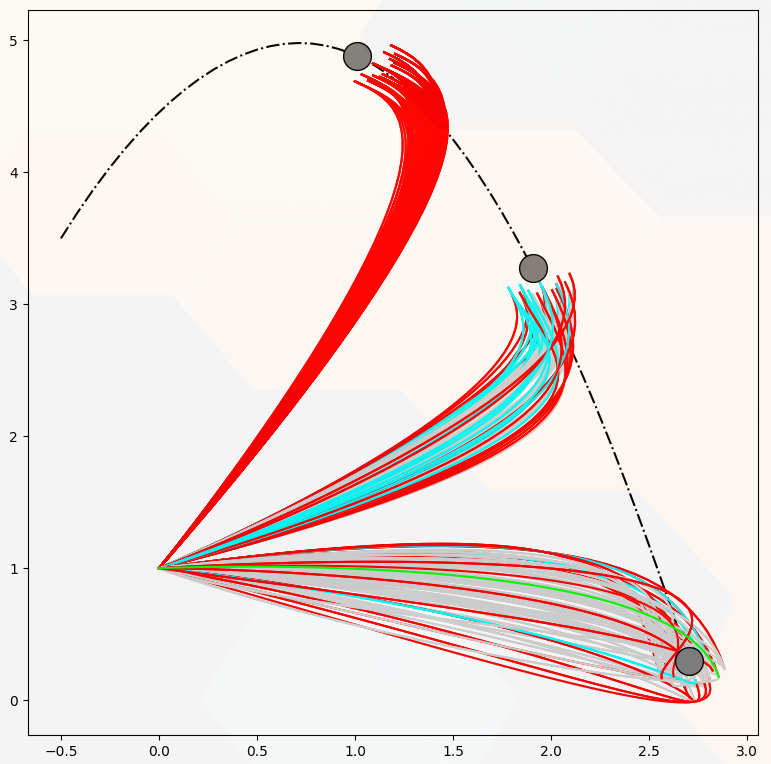
\includegraphics[width=0.7\linewidth]{generation_example.png}
% 	\caption{Generated trajectories for different final states and time horizons.}
    
% \end{figure}
\section{Feasibility of Trajectories}
\label{sec:feasibility}
In the previous section, the trajectory generation approach was presented and the relation between the state trajectory and the system inputs has been established.
Still, we have to ensure the trajectory is actually feasible regarding the translational constraints in \Cref{eq:translational-constraints}, as the constraints are generally neglected during the generation stage.
The same applies to the input feasibility.
Since these constraints are not inherent to the generation stage, they can be considered as feasibility tests, classifying the given trajectory as feasible or not. 

\subsection{Input Feasibility}
\label{sec:input-feasibility}

We can split the problem of input feasibility into two subproblems, namely, thrust feasibility and body rate feasibility. The thrust feasibility check ensures that the vehicle does not exceed its thrust capabilities denoted by $\fmin$ for the minimum and $\fmax$ for the maximum thrust it can generate.
We formulate the thrust constraints as
\begin{equation}
	\label{eq:thrust-limits}
	\unit[0]{N} \leq f_\text{min} \leq f \leq f_\text{max}
	.
\end{equation}
The body rate feasibility check declares a given state trajectory feasible if
\begin{equation}
	\label{eq:body-rates-limit}
	\left\lVert\omeb\right\rVert
	\leq
	\omega_\text{max}
\end{equation}
is guaranteed to be valid over the whole trajectory.

Both checks are applied on the trajectory per axis with sufficient but not necessary criteria for both, feasibility and infeasibility. As a consequence, there might be feasible (as well as infeasible) trajectories that might be classified as indeterminable. The checks are applied recursively on subsections of the whole interval $\left[0,T\right]$ in case they cannot classify the section as provably feasible or unfeasible.

\subsubsection{Thrust Input Feasibility}
% \begin{itemize}
% 	\color{red}
% 	\item stress out, that feasibility criterium is quite coarse -> feasible solution might be classified as indeterminable
% \end{itemize}
We consider the interval 
\begin{equation}
	\mathcal{T} = \left[\tau_1,\tau_2\right] \subseteq \left[0,T\right]
	,
\end{equation}
for which the thrust feasibility criterion in \Cref{eq:thrust-limits} is fulfilled if and only if
\begin{align}
	\label{eq:thrust-feasibility-equivilency-max}
	\max_{t \in \mathcal{T}} f(t)^2
	&\leq
	f_\text{max}^2 \\
	\label{eq:thrust-feasibility-equivilency-min}
	\min_{t \in \mathcal{T}} f(t)^2
	&\geq
	f_\text{min}^2
	.
\end{align}

By squaring \Cref{eq:trajectory-thrust}, we can write the squared thrust in per-axis notation
\begin{equation}
	\label{eq:thrust-squared-per-axis}
	f^2 = 
	\left\lVert
	\left(m + X_{\dot{u}}\right) \pbpp + X_u \pbp
	\right\rVert^2
	= 
	\sum_{k=1}^{3}
	\left(\left(m + X_{\dot{u}}\right)\ppp_k + X_u \pp_k \right)^2
\end{equation}
and bound the thrust conservatively by summation over the per axis extrema
\begin{align}
	\label{eq:fmax-per-axis}
	\max_{t \in \mathcal{T}} f(t)^2
	&\leq
	\sum_{k=1}^{3}
	\max_{t \in \mathcal{T}}
	\left(
		\left(m + X_{\dot{u}}\right)
		\ppp_k
		+ X_u \pp_k
	\right)^2, \\
	\label{eq:fmin-per-axis}
	\min_{t \in \mathcal{T}} f(t)^2
	&\geq
	\sum_{k=1}^{3}
	\min_{t \in \mathcal{T}}
	\left(
		\left(m + X_{\dot{u}}\right)
		\ppp_k
		+ X_u \pp_k
	\right)^2
	.
\end{align}

Moreover, we denote the maximum and minimum of the per axis thrust as \fmaxaxis and \fminaxis, respectively %\todo{Hier ist im Unterschied zu Mueller eine kubische Funktion fuer die Nullstellen zu loesen} 
and write the extrema in \Cref{eq:fmax-per-axis,eq:fmin-per-axis} as
\begin{align}
	\max_{t \in \mathcal{T}}
	\left(
		\left(m + X_{\dot{u}}\right)
		\ppp_k
		+ X_u \pp_k
	\right)^2
	&= 
	\max\left\{\fmaxaxis^2, \fminaxis^2\right\} \\
	\min_{t \in \mathcal{T}}
	\left(
		\left(m + X_{\dot{u}}\right)
		\ppp_k
		+ X_u \pp_k
	\right)^2
	&=
	\begin{cases}
		\min\left\{\fmaxaxis^2, \fminaxis^2\right\}
		& \text{if } \fmaxaxis\cdot\fminaxis > 0 \\
		0
		& \text{otherwise}
	\end{cases}
\end{align}

A sufficient criterion, rendering the trajectory infeasible, is
\begin{equation}
	\label{eq:sufficient-infeasible-thrust}
	\max\left\{\fmaxaxis^2, \fminaxis^2\right\}
	> \fmaxsquare
	,
\end{equation}
whereas a sufficient criterion for feasibility with respect to the thrust input is if both
\begin{align}
	\label{eq:sufficient-feasible-thrust-max}
	\sum_{k=1}^{3}
	\max_{t \in \mathcal{T}}
	\left\{\fmaxaxis^2, \fminaxis^2\right\}
	& \leq
	\fmaxsquare, \\
	\label{eq:sufficient-feasible-thrust-min}
	\sum_{k=1}^{3}
	\min_{t \in \mathcal{T}}
	\left\{\fmaxaxis^2, \fminaxis^2\right\}
	& \geq
	\fminsquare
\end{align}
hold. 
Note that it might be the case, that neither \Cref{eq:sufficient-infeasible-thrust} nor \Cref{eq:sufficient-feasible-thrust-max,eq:sufficient-feasible-thrust-min} hold. This does not necessarily mean that the section has to be infeasible. 
Even though the highest order term $\pp_k$ is of fourth order due to velocity dependent damping opposed to the \ac{uav} application in \cite{MuellerHehn15}, where it is of order three, we can still consider the per axis criteria as computationally efficient. 
Finding the extrema of a fourth order polynomial comes down to finding the roots of a third order polynomial, for which a closed form solution exists. Additionally, to find the extrema for the interval $\mathcal{T}$ it is sufficient to solve it once for the whole duration of the trajectory. Subsequently, we check for each interval $\mathcal{T}$, if the candidate for a local extremum lies within $\mathcal{T}$ and find the global extrema for $\mathcal{T}$ by comparing the thrusts of the respective candidate with the thrust values on the boundaries of $\mathcal{T}$. We can conclude, that in the best case, i.\,e. no local extremum candidate lies within $\mathcal{T}$, two function evaluations of a quartic polynomial are required. Whereas, for the worst case, i.\,e. all local extremum candidates lie within $\mathcal{T}$, five evaluations are required.

To obtain the thrust function in terms of the state trajectory parameters $\alpha$, $\beta$, and $\gamma$, we plug \Cref{eq:optimal-trajectory-per-axis} into \Cref{eq:trajectory-thrust}, which yields
\begin{equation}
	\begin{aligned}
		f ={}
		&\frac{X_u \alpha}{24} t^4
		+ \frac{X_u \beta + \left(m+X_{\dot{u}}\right)}{6} t^3
		+ \frac{X_u \gamma + \left(m + X_{\dot{u}}\right)}{2} t^2 \\
		& + \left(
			X_u a_0 + \left(m + X_{\dot{u}}\right) \gamma
		\right) t
		+ X_u v_0
		+ \left(m + X_{\dot{u}}\right) a_0
\end{aligned}
\end{equation}
per axis.

\begin{algorithm}
    \caption{CheckThrustFeasibility}
    \label{alg:thrust-feasibility}
	\begin{algorithmic}[1]
		\Function{CheckThrustFeasibility}{$\fmin$, $\fmax$, $\tau_1$, $\tau_2$}
		\If{$\tau_2 - \tau_1 < \tau_{\min}$}
		\Comment{Termination criterion to limit recursion depth}
			\State \textbf{return} indeterminable
		\EndIf
		% \LeftComment check the boundaries of the interval explicitly
		% \State $f_1 \gets$ \Call{Max}{\Call{Thrust}{$\tau_1$}, \Call{Thrust}{$\tau_2$}}
		% \State $f_2 \gets$ \Call{Min}{\Call{Thrust}{$\tau_1$}, \Call{Thrust}{$\tau_2$}}
		% \If{$f_1 > \fmax$}
		% 	\State \textbf{return} infeasible
		% \ElsIf{$f_2 < \fmin$}
		% 	\State \textbf{return} infeasible
		% \EndIf
		\State $\Sigma_{\min}^2 \gets 0$
		\Comment{Sum of $\min(f^2)$ over all axes}
		\State $\Sigma_{\max}^2 \gets 0$
		\Comment{Sum of $\max(f^2)$ over all axes}
		\For{all axes}
			\State $f_1, f_2 \gets \Call{MinMaxThrustOfAxis}{\tau_1, \tau_2}$
			\If{\Call{Max}{$f_1^2,f_2^2$} $> \fmax$} \Comment{a single axis exceeds $\fmax$}
				\State \textbf{return} infeasible
			\EndIf
			\If{$f_1 \cdot f_2 < 0$}
				\State $\Sigma_{\min}^2 \gets \Sigma_{\min}^2$
			\Else
				\State $\Sigma_{\min}^2 \gets \Sigma_{\min}^2 + \Call{Min}{f_1^2, f_2^2}$
			\EndIf
			\State $\Sigma_{\max}^2 \gets \Sigma_{\max}^2 + \Call{Max}{f_1^2, f_2^2}$
		\EndFor
		\If{$\Sigma_{\max}^2 < \fminsquare$}
		\Comment{Apply the infeasibility criterion}
			\State \textbf{return} infeasible
		\ElsIf{$\Sigma_{\min}^2 > \fmaxsquare$}
			\State \textbf{return} infeasible
		\EndIf
		\If{$\Sigma_{\max}^2 \leq \fmaxsquare$ and $\Sigma_{\min}^2 \geq \fminsquare$}
		\Comment{Apply the feasibility criterion}
			\State \textbf{return} feasible
		\Else \Comment{Test feasibility recursively on subintervals}
			\State $\tau_{\text{m}} \gets (\tau_1 + \tau_2) / 2$
			\If {\Call{CheckThrustFeasibility}{$\fmin,\fmax,\tau_1,\tau_{\text{m}}$} $=$ feasible}
				\State \textbf{return} \Call{CheckThrustFeasibility}{$\fmin,\fmax,\tau_{\text{m}},\tau_2$}
			\Else
				\State \textbf{return} infeasible
			\EndIf
		\EndIf
		\EndFunction
	\end{algorithmic}
\end{algorithm}

\subsubsection{Body Rates Input Feasibility}
We can formulate an upper bound on the body rates by applying the vector induced euclidean norm $\left\lVert\Rb\right\rVert \leq 1$ on \Cref{eq:body-rate-relation}, yielding
\begin{equation}
	\label{eq:body-rates-bound}
	\omega_3^2 + \omega_2^2 \leq
	\frac{1}{f^2}
	\left\lVert
		\left(
			m + X_{\dot{u}}
		\right) \pbppp + X_u \pbpp
	\right\rVert^2
	.
\end{equation}
Moreover, a conservative upper bound of \Cref{eq:body-rates-bound} in per axis notation denoted as $\bar{\omega}^2$ can be written with \Cref{eq:thrust-squared-per-axis} as
\begin{equation}
	\omega_2^2 + \omega_3^2
	\leq
	\bar{\omega}^2
	=
	\frac{
		\sum_{k=1}^{3}
		\max_{t \in \mathcal{T}}
		\left(
			\left(
				m + X_{\dot{u}}
			\right)\dddot{p}_k + X_u \ddot{p}
		\right)^2
	}{
		\sum_{k=1}^{3}
		\min_{t \in \mathcal{T}}
		\left(
			\left(m + X_{\dot{u}}\right)\ppp_k
			+ X_u \pp_k
		\right)^2
	}
	.
\end{equation}
Furthermore, simplifying with \Cref{eq:sufficient-feasible-thrust-min} and defining $\xi_k = \left(m + X_{\dot{u}}\right)\dddot{p}_k + X_u \ddot{p}$, results in
\begin{equation}
	\bar{\omega}^2 =
	\frac{
		\sum_{k=1}^{3}
		\max_{t \in \mathcal{T}}
		\xi_k^2
	}{
		\sum_{k=1}^{3}
		\min_{t \in \mathcal{T}}
		\left\{\fmaxaxis^2, \fminaxis^2\right\}
	}
	.
\end{equation}
Hereby, the minimum and maximum of $\xi_k$ is denoted as \ximaxaxis and \ximinaxis, respectively. With
\begin{equation}
	\max_{t \in \mathcal{T}}
	\left(
		\left(
			m + X_{\dot{u}}
		\right)
		\dddot{p}_k + X_u \ddot{p}
	\right)^2 =
	\max_{t \in \mathcal{T}}
	\left\{
		\ximaxaxis^2, \ximinaxis^2
	\right\}
	,
\end{equation}
we formulate the feasibility criterion with respect to the body rates
\begin{equation}
	\label{eq:body-rates-criterion-per-axis}
	\bar{\omega}^2
	=
	\frac{
		\sum_{k=1}^{3}
		\max_{t \in \mathcal{T}}
		\left\{
			\ximaxaxis^2, \ximinaxis^2
		\right\}
	}{
		\sum_{k=1}^{3}
		\min_{t \in \mathcal{T}}
		\left\{\fmaxaxis^2, \fminaxis^2\right\}
	}
	\leq
	\omegamaxsquare
	.
\end{equation}
This body rate feasibility criterion is analogue to the upper bound criterion for the thrust feasibility in \Cref{eq:sufficient-feasible-thrust-max}. If \Cref{eq:body-rates-criterion-per-axis} does not hold, the tested interval $\mathcal{T}$ is split in half and the feasibility criterion is applied recursively on both subintervals, subsequently.


\subsection{Translational Constraints Feasibility}
At this stage, we can check if a trajectory meets the requirements for being classified as input feasible as presented in \Cref{sec:input-feasibility}. Still, there is no guarantee, the trajectory will not violate the translational constraints formulated in \Cref{eq:translational-constraints}.

\subsubsection{Position Feasibility}
\label{sec:position-feasibility}
We can formulate position constraints as planes. We define the allowable side of the plane by a normal vector $\nb_{\text{p}}$. We call this kind of positional constraints \textit{wall constraints}. These wall constraints can be used to encode constraints due to local conditions, such as the water surface or the walls of a confined environment, that an underwater vehicle is not allowed or able to cross. Feasibility has to be tested for critical points only. The critical points are those meeting the sufficient criterion for being at a minimal distance to the plane encoding the wall constraint. We find these critical points by finding the roots of $\pp_{\text{n}}(t) = \nb_{\text{p}}^\top \, \pbp(t)$.
The constraints then read
\begin{equation}
	\mathcal{C}_{\text{crit}} =
	\left\{
		t \in \left[ 0, T \right]
		\,\mid\, \pp_{\text{n}}(t) = 0
	\right\}
	\cup
	\left\{0,T\right\}
\end{equation}
Furthermore, the trajectory is feasible with respect to the position constraints if and only if
\begin{equation}
	\label{eq:position-feasibility-criterion}
	\nb_\text{p}^\top
	\left(
		\pbo(t) - \pbo_{\text{p}}
	\right)
	> 0
	\,\forall\, t \in \mathcal{C}_{\text{crit}}
	,
\end{equation}
with $\pbo_{\text{p}}$ denoting an arbitrary point on the plane defining the wall constraint. Geometrically interpreted, we can regard $\pp_{\text{n}}$ as the velocity projected onto the normal direction of the plane given by $\nb_{\text{p}}$.

The position is a quintic polynomial, as we can see in \Cref{eq:optimal-trajectory-per-axis}. Thus, computing $\mathcal{C}_{\text{crit}}$ is done by solving the roots of the fourth-order polynomial $\pp_{\text{n}}$. Therefore, the feasibility check is carried out by evaluating the left-hand side of \Cref{eq:position-feasibility-criterion} at least twice and at most six times per axis. This is similar to the input feasibility checks presented in \Cref{sec:input-feasibility} with the difference that no recursion is needed, though.



\section{Collision Avoidance}\label{sec:collision-avoidance}
As for the translational constraints and the input feasibility, collision avoidance is not inherent to the generation of trajectories, but is applied as a test afterwards. Trajectories failing the test are discarded.
Obstacle avoidance can be added to the trajectory planning straightforwardly by extending the position feasibility test in \Cref{sec:position-feasibility}.
Instead of checking for a collision with a single predefined plane, the position check is performed recursively on subintervals of $\left[0, T\right]$.
For each recursion, a plane separating the section of the trajectory from the convex obstacle $\mathcal{O}$ is defined.
The position feasibility check is performed and if the whole section lies on the allowable side of separating plane, i.e. in the direction away from the object, the section is declared feasible.
Otherwise, the check is performed recursively on the subinterval including the intersection with the separating plane.
The interested reader may refer to \cite{Bucki19} for an exhaustive analysis of such a collision avoidance algorithm in the domain of aerial vehicles.
The pseudocode describing an algorithm performing the collision feasibility test can be seen in \Cref{alg:collision-detection}.
\begin{algorithm}
    \caption{Collision Detection based on \cite{Bucki19}}
    \label{alg:collision-detection}
	\begin{algorithmic}[1]
		\Require $\pbo(0),\pbo(T) \notin \mathcal{O}$
		\Function{CollisionFeasibility}($\tau_{\min}$)
			\If{not $\pbo(0),\pbo(T) \notin \mathcal{O}$}
				\State \textbf{return} infeasible
			\EndIf
			\State \textbf{return}
			\Call{CollisionCheck}{$0, T$}
		\EndFunction
		\Function{CollisionCheck}{$\tau_1, \tau_2$}
		\State $\tau_{\text{mid}} \gets (\tau_1 + \tau_2) / 2$
		\If{$\pbo(\tau_{\text{mid}}) \in \mathcal{O}$}
			\State \textbf{return} infeasible
		\ElsIf{$\tau_2 - \tau_1 < \tau_{\min}$}
			\State \textbf{return} indeterminable
		\EndIf
		\State $\pbo_{\text{p}}, \nb_{\text{p}} \gets$
		\Call{GetSeparatingPlane}{$\pbo(\tau_{\text{mid}}),\mathcal{O}$}
		\State $\mathcal{C}_{\text{crit}} \gets
		\left\{
			t \in \left[ \tau_{\text{mid}}, \tau_2 \right]
			\,\mid\, \pp_{\text{n}}(t) = 0
		\right\}$ in ascending order
		\For{$t_i$ in $\mathcal{C}_{\text{crit}}$, skipping $\tau_{\text{mid}}$}
			\If{$\nb_\text{p}^\top
				\left(
					\pbo(t_i) - \pbo_{\text{p}}
				\right)
				\leq 0$}
				\State result $\gets$ \Call{CollisionCheck}{$t_{i-1},\tau_2$}
				\If{result = feasible}
					\State \textbf{break}
				\Else
					\State \textbf{return} result
					\Comment{either infeasible or indeterminable}
				\EndIf
			\EndIf
		\EndFor
		\State $\mathcal{C}_{\text{crit}} \gets
		\left\{
			t \in \left[ \tau_1, \tau_{\text{mid}}\right]
			\,\mid\, \pp_{\text{n}}(t) = 0
		\right\}$ in descending order
		\For{$t_i$ in $\mathcal{C}_{\text{crit}}$, skipping $\tau_{\text{mid}}$}
			\If{$\nb_\text{p}^\top
			\left(
				\pbo(t_i) - \pbo_{\text{p}}
			\right)
			\leq 0$}
				\State \textbf{return} \Call{CollisionCheck}{$\tau_1, \tau_{\text{mid}}$}
			\EndIf
		\EndFor
		\State \textbf{return} feasible
		\EndFunction
	\end{algorithmic}
\end{algorithm}

The recursion depth of \Cref{alg:collision-detection} is limited by $\tau_{\min}$.
If an examined section of the trajectory bounded by the time interval $\left[\tau_1, \tau_2\right]$ becomes small enough that $\tau_2 - \tau_1 < \tau_{\min}$, the trajectory is declared indeterminable.
Computation time wise, we can expect the choice of $\tau_{\min}$ to have a significant influence for indeterminable trajectories.
This is, because $\tau_{\min}$ limits the recursion depth in case no subinterval has been declared infeasible yet, nor could feasibility be guaranteed for the whole interval $\left[0, T\right]$.
Choosing $\tau_{\min}$ larger reduces the time required in case feasibility could not be decided upon before splitting the interval in smaller sections than $\tau_{\min}$.
On the other hand, choosing $\tau_{\min}$ smaller could result in trajectories being declared as feasible, that would have been discarded as indeterminable otherwise.

Note that we are not restricted to static obstacles by this approach of obstacle avoidance. We define the trajectory of the relative position of the vehicle to the obstacle as
\begin{equation}
	\pbs(t) = \pbo(t) - \pbo_{\mathcal{O}}(t)
	,
\end{equation}
where $\pbo_{\mathcal{O}}(t)$ denotes the obstacle's trajectory. Instead of performing the collision check for $\pbo$, we do it for $\pbs$. In general, $\pbo_{\mathcal{O}}$ and consequently $\pbs$ could be arbitrary functions of time.
But choosing them not to be a polynomial of order at most five, would render the collision avoidance significantly less computational efficient. Hence, we assume the trajectories being of at most order five, and the collision avoidance being performable by solving roots of quartic polynomials.

% \textcolor{red}{\Cref{fig:polynomial_example} wants to be referenced}

% \begin{figure}
%     \centering
%     \begin{tikzpicture}
%     \begin{axis}[
%             xmin=-2,xmax=1,
%             ymin=-3,ymax=3,
%             grid=both,
%             ]
%             \addplot [domain=-0.5:3.5,samples=50]({-1.083 * x^3 + 5.25 * x^2 -6.67*x + 1},{0.167 * x^3 - 0.25 * x^2 + 0.583 *x - 2}); 
%     \end{axis}
%     \caption{\textcolor{red}{Was zeigen wir hier?}}
%     \label{fig:polynomial_example}
% \end{tikzpicture}
% \end{figure}


\section{Control}
\label{sec:control}
% \begin{itemize}
% 	\color{red}
% 	%\item one could use the min jerk trajectory approach simply for generation -> feed-back control to keep the vehicle on track
% 	%\item computational efficiency and real-time capability of approach enables trajectory generation to be used for implicit feedback. Regenerate trajectories in each control time step.
% 	%\item body rates will change rather slowly compared to quadrocopters -> instead of using body rates as in MuellerHehn15, use target attitude and attitude control (actually the body rates are derived from a target attitude anyway)
% \end{itemize}
While we attended to the generation and planning of trajectories, as well as the question of feasibility regarding vehicle dynamics, translational constraints and collision avoidance in the previous sections, this section is about tracking the obtained trajectories.

The general control architecture implements the inner-outer loop control scheme as depicted in \Cref{fig:inner-outer-loop-feedback-control}.
\begin{figure}[tb]
	\centering
	\begin{tikzpicture}

    \scriptsize

    \def\blockheight{1.5cm}
    \def\blockwidth{1.5cm}
    \def\xshiftblocks{0cm}
    \def\yshifttwolines{0.3cm}  % yshift for connecting lines between blocks when two lines above each other are used
    \def\yshiftthreelines{0.4cm}  % yshift for connecting lines between blocks when three lines above each other are used
    \def\yshiftfourlines{0.4cm}
    \def\yshiftbelowvehiclefirst{-0.5cm}
    \def\yshiftbelowvehicleoffset{-0.2cm}
    \def\yshiftaboveblocks{0.5cm}
    \def\xshiftfirstuintomixer{-0.8cm}    

        % Blocks
		\node[draw, fill=lightgray, semithick, rectangle, minimum width=\blockwidth, minimum height=\blockheight, align=center] (generator) at (0,0) {Trajectory\\Generator};
		\node[draw, fill=lightgray, semithick, rectangle, minimum width=\blockwidth, minimum height=\blockheight, align=center, right= of generator, xshift=\xshiftblocks] (trackingcontroller) {Trajectory\\Tracking\\Controller};
		\node[draw, fill=lightgray, semithick, rectangle, minimum width=\blockwidth, minimum height=\blockheight, align=center, right= of trackingcontroller, xshift=\xshiftblocks] (attitudecontroller) {Attitude\\Controller};
        \node[draw, fill=lightgray, semithick, rectangle, minimum width=\blockwidth, minimum height=\blockheight, align=center, right= of attitudecontroller, xshift=\xshiftblocks] (ratecontroller)  {Rate\\Controller};
        \node[draw, fill=lightgray, semithick, rectangle, minimum width=\blockwidth-0.5cm, minimum height=2cm, align=center, right= of ratecontroller, xshift=\xshiftblocks] (mixer)  {Mixer};
        \node[draw, fill=lightgray, semithick, rectangle, minimum width=\blockwidth-0.3cm, minimum height=\blockheight, align=center, right= of mixer, xshift=\xshiftblocks+0.7cm] (vehicle)  {Vehicle};
		
        % trajectory generator - trajectory tracking controller
		\draw[-stealth] (generator.east) -- (trackingcontroller.west) node[midway, above] {$\bm{\sigma}_{\text{des}}$};

        % trajectory tracking controller - attitude controller
        \draw[-stealth] ([yshift=\yshifttwolines]trackingcontroller.east) -- ([yshift=\yshifttwolines]attitudecontroller.west) node[midway, above] {$\bm{f}_{\text{des}}$};
        \draw[-stealth] ([yshift=-\yshifttwolines]trackingcontroller.east) -- ([yshift=-\yshifttwolines]attitudecontroller.west) node[midway, above] {$\bm{\phi}_{\text{des}}$};
        
        % attitude controller - rate controller
        \draw[-stealth] (attitudecontroller.east) -- (ratecontroller.west) node[midway, above] {$\bm{\omega}_{\text{des}}$};

        % rate controller - mixer
		\draw[-stealth] ([yshift=\yshiftthreelines]ratecontroller.east) -- ([yshift=\yshiftthreelines]mixer.west) node[midway, above] {$u_2$};
        \draw[-stealth] ([yshift=0cm]ratecontroller.east) -- ([yshift=0cm]mixer.west) node[midway, above] {$u_3$};
        \draw[-stealth] ([yshift=-\yshiftthreelines]ratecontroller.east) -- ([yshift=-\yshiftthreelines]mixer.west) node[midway, above] {$u_4$};

        % mixer - vehicle
        \draw[-stealth] ([yshift=\yshiftfourlines]mixer.east) -- ([yshift=\yshiftfourlines]vehicle.west) node[midway, above, align=center] {ESC\\commands};
        \draw[-stealth] ([yshift=1/3*\yshiftfourlines]mixer.east) -- ([yshift=1/3*\yshiftfourlines]vehicle.west) node[midway, above] {};
        \draw[-stealth] ([yshift=-1/3*\yshiftfourlines]mixer.east) -- ([yshift=-1/3*\yshiftfourlines]vehicle.west) node[midway, above] {};
        \draw[-stealth] ([yshift=-\yshiftfourlines]mixer.east) -- ([yshift=-\yshiftfourlines]vehicle.west) node[midway, below] {};

        % vehicle - below all other blocks
        \draw[-stealth] ([xshift=-0.2cm]vehicle.south) -- ++(0, \yshiftbelowvehiclefirst) -- ([yshift=\yshiftbelowvehiclefirst]ratecontroller.south) -- (ratecontroller.south) node[midway, right] {$\omeb, \omebp$};
        \draw[-stealth] ([xshift=-0cm]vehicle.south) -- ++(0, \yshiftbelowvehiclefirst+\yshiftbelowvehicleoffset) -- ([yshift=\yshiftbelowvehiclefirst+\yshiftbelowvehicleoffset]attitudecontroller.south) -- (attitudecontroller.south) node[midway, right] {$\qb$};
        \draw[-stealth] ([xshift=0.2cm]vehicle.south) -- ++(0, \yshiftbelowvehiclefirst+2*\yshiftbelowvehicleoffset) -- ([yshift=\yshiftbelowvehiclefirst+2*\yshiftbelowvehicleoffset]trackingcontroller.south) -- (trackingcontroller.south) node[midway, right] {$\pbo,\pbp$};
        \draw[-stealth] ([yshift=\yshiftbelowvehiclefirst+2*\yshiftbelowvehicleoffset]trackingcontroller.south) -- ([yshift=\yshiftbelowvehiclefirst+2*\yshiftbelowvehicleoffset]generator.south) -- (generator.south) node[midway, right] {$\pbo,\pbp,\pbpp$};

        % trajectory tracking controller - mixer (above blocks)
        \draw[-stealth] ([xshift=0.3cm]trackingcontroller.north) -- ++(0, \yshiftaboveblocks) -- ([xshift=\xshiftfirstuintomixer, yshift=\yshiftaboveblocks+0.5*\blockheight]mixer.west) -- ([xshift=\xshiftfirstuintomixer, yshift=2*\yshiftthreelines]mixer.west) -- ([yshift=2*\yshiftthreelines]mixer.west) node[midway, above] {$u_1$};

	\end{tikzpicture}
	\caption{Overview of the control loops.} %The outer control loop consists of the trajectory tracking controller that outputs a desired thrust vector $\bm{f}_{\text{des}}$ and a roll angle $\bm{\phi}_{\text{des}}$, fully defining a desired state of the vehicle, allowing the vehicle to follow the given trajectory. This is then fed into the high-rate, low-level attitude controller. This controller outputs a desired resulting attitude, which is then achieved using the body rate controller. 
	\label{fig:inner-outer-loop-feedback-control}
\end{figure}
The authors in \cite{Maurya09} demonstrated the viability of this approach for marine vehicles. The basic idea is to divide the problem of trajectory into easier-to-solve subproblems. By inner loops, we refer to the low-level dynamic control loops consisting of attitude or body rate controllers. The design and tuning of these inner loops are highly dependent on the vehicle dynamics. The outer control loops, for example, a position, path, or trajectory tracking controller, can be considered as kinematic control loops. They are by design decoupled from vehicle dynamics under the assumption that the inner control loops are fast enough to reach the target value instantaneously from the perspective of the outer loop. This is equivalent to the assumption in \Cref{sec:thruster-model} that the thruster dynamics compared to the \ac{uauv} dynamics are sufficiently fast to be negligible. As a result, we have a fast-slow separation from the inner to the outer loop, i.e. the inner loops run with a significantly higher frequency than the outer ones.


\subsection{Body Rate Control}
The body rate controller represents the innermost control loop.

We define the error of the angular velocity and acceleration in the body-fixed frame $\mathcal{B}$
\begin{equation}
	\vangerror = \vangbody - \vangdesiredbody \quad \text{and} \quad
	\aangerror = \aangbody - \aangdesiredbody
	,
\end{equation}
and the control law for controlling $\vangbody$, reading
\begin{align}
	\begin{bmatrix}
		u_2 \\ u_3 \\ u_4
	\end{bmatrix}
	=
	\KpBodyRate \vangerror
	&+ \KiBodyRate \int_{}^{t} \vangerror(\tau)\text{d}\tau
	+ \KdBodyRate \aangerror \\\nonumber
	&+\underbrace{
		\vangdesiredbody \times \Jbs \vangdesiredbody
		+ \Domegaadded \vangdesiredbody
		- \vlinbody \times \Mbs \vangdesiredbody
	}_{\text{feed forward}}
	,
\end{align}
%\todo{add p and d term and we have pid with feedfoward. }
where the feed forward terms are based on vehicle dynamics in \Cref{eq:eom-rotational-with-input}. The control law displays a PID-Controller with feed forward term, where $\KpBodyRate$, $\KiBodyRate$ and $\KdBodyRate$ are diagonal matrices denoting the proportional, integral and derivative gain, respectively.

We set $\aangdesiredbody = \unit[0]{rad/s^2}$ and observe that the input for the body rate controller is $\vangdesiredbody$. We will see in \Cref{sec:implicit-feedback-control} the usefulness of this for the implicit feedback control scheme in the context of the trajectory generation system, given the inner-outer loop assumptions hold.

\subsection{Attitude Control}
The attitude controller is the next controller upstream of the body rate controller. Hence, we consider it to be a kinematic controller with a desired body rate $\vangdesiredbody$ as output, instead of the vehicle's system inputs $\inputbody$. We define the desired thrust axis as the controller's input 
\begin{equation}
	\exdesiredbodyinworld =
	\frac{\thrustdesiredworld}{
		\left\lVert\thrustdesiredworld\right\rVert
	}
\end{equation}
and the current thrust axis that is equivalent to 
\begin{equation}
	\exbodyinworld = \qactual \odot \eb_1
	,
\end{equation}
where $\qactual \odot \eb_1$ denotes the rotation of the vector $\eb_1$ by the quaternion $\qactual$, while $\qactual$ is the current attitude of the vehicle.

This controller computes a desired attitude given by the quaternion $\qdesired$ and computes the required body rates $\vangdesiredbody$ that result in rotating the vehicle to the desired attitude. For this, we define the error of the attitude as
\begin{equation}
	\label{eq:qerror}
	\qerror = \qactual^{-1} \cdot \qdesired
	.
\end{equation}
Furthermore, the alignment of $\exdesiredbodyinworld$ and $\exbodyinworld$ constraints two of the three rotational degrees of freedom of the vehicle, namely pitch and yaw.
On the other hand, the rotation around the roll axis $\exbodyinworld$ can be chosen freely.

The quaternion-based control law
\begin{equation}
	\label{eq:control-law-attitude}
	\vangdesiredbody = 
	\frac{2}{\tau}
	\text{sgn}(q_{\text{e},0})
	\qb_{\text{e},1:3}
\end{equation}
is globally asymptotically stable and fits the architecture of inner-outer loops \cite{Mayhew11,Brescianini13}, which is desirable in the context of agile maneuvering. The parameter $\tau$ can be interpreted as first-order time constant of the attitude controller. In practice, too small or too large values may lead to bad control performance \cite{Brescianini13}. Therefore, an appropriate value has to be determined by tuning of the controller.

The axis-angle representation of the rotation aligning $\exbodyinworld$ and $\exdesiredbodyinworld$ is given by
\begin{equation}
	\rotationaxisworld = \frac{
		\exbodyinworld \times \exdesiredbodyinworld
	}{
		\left\lVert
			\exbodyinworld \times \exdesiredbodyinworld
		\right\rVert
	}
	\quad \text{and} \quad
	\alpha = \arccos
	\left(
		\exbodyinworld^\top \exdesiredbodyinworld
	\right)
	.
\end{equation}
We construct the error quaternion for pitch and yaw straightforwardly from the angle-axis representation 
\begin{equation}
	\qerrorPY = 
	\begin{cases}
		\begin{bmatrix}
			\cos(\frac{\alpha}{2}) \\
			\sin(\frac{\alpha}{2}) \rotationaxisworld
		\end{bmatrix} &\text{if } \alpha \neq 0 \\
		\begin{bmatrix}
			1 & 0 & 0 & 0
		\end{bmatrix}^\top
		& \text{else.}
	\end{cases}
\end{equation}
Note that the way we construct the rotation axis, it will never cause a rotation around the vehicle's roll axis as $\exdesiredbodyinworld \perp \exbodyinworld \times \exdesiredbodyinworld$ per definition of the cross product. 

The desired attitude aligning $\exdesiredbodyinworld$ and $\exbodyinworld$ reads
\begin{equation}
	\qdesiredPY = \qactual \cdot \qerrorPY
	.
\end{equation}

We introduce the intermediate coordinate system $\mathcal{C}$, that is rotated to $\mathcal{W}$ around $bm{x}_{\mathcal{W}}$ by the $\rolldesired$. 
Subsequently, we can determine $\eydesiredbodyinworld$ and thereby $\ezdesiredbodyinworld$, so that we achieve the alignment of $\exdesiredbodyinworld$ with the desired roll angle according to \cite{Mayhew11}
\begin{align}
	\eydesiredbodyinworld = 
	\frac{\ezinterinworld \times \exdesiredbodyinworld}{
		\left\lVert
			\ezinterinworld \times \exdesiredbodyinworld
		\right\rVert
	}\quad \text{and}
	\ezdesiredbodyinworld =
	\exdesiredbodyinworld \times \eydesiredbodyinworld.
\end{align}
We can construct $\qdesiredfull$ from the three desired body axes and define
\begin{equation}
	\qmix = \qdesiredPY^{-1} \cdot \qdesiredfull =
	\begin{bmatrix}
		\cos\left(\frac{\anglemix}{2}\right) \\
		\sin\left(\frac{\anglemix}{2}\right) \\
		0 \\
		0
	\end{bmatrix},
\end{equation}
as the rotation between $\qdesiredPY$ and $\qdesiredfull$ with $\anglemix$ being the rotation angle. We can scale $\anglemix$ by $p \in \left[0,1\right]$ to determine the fraction of $\rolldesired$ to consider for the desired attitude
\begin{equation}
	\label{eq:qdesired}
	\qdesired = \qdesiredPY
	\begin{bmatrix}
		\cos\left(p\frac{\anglemix}{2}\right) \\
		\sin\left(p\frac{\anglemix}{2}\right) \\
		0 \\
		0
	\end{bmatrix}
	.
\end{equation}
Finally, we plug  \Cref{eq:qdesired} into \Cref{eq:qerror} in order to apply the control law in \Cref{eq:control-law-attitude}.



\subsection{Implicit Feedback Control}
\label{sec:implicit-feedback-control}

\begin{figure}[tb]
	\centering
	\begin{tikzpicture}

    \scriptsize

    \def\blockheight{1.5cm}
    \def\blockwidth{1.5cm}
    \def\xshiftblocks{0cm}
    \def\yshifttwolines{0.3cm}  % yshift for connecting lines between blocks when two lines above each other are used
    \def\yshiftthreelines{0.4cm}  % yshift for connecting lines between blocks when three lines above each other are used
    \def\yshiftfourlines{0.4cm}
    \def\yshiftbelowvehiclefirst{-0.5cm}
    \def\yshiftbelowvehicleoffset{-0.2cm}
    \def\yshiftaboveblocks{0.5cm}
    \def\xshiftfirstuintomixer{-0.8cm}    

        % Blocks
		\node[draw, fill=lightgray, semithick, rectangle, minimum width=\blockwidth, minimum height=\blockheight, align=center] (generator) at (0,0) {Trajectory\\Generator};
        \node[draw, fill=lightgray, semithick, rectangle, minimum width=\blockwidth, minimum height=\blockheight, align=center, right= of generator, xshift=\xshiftblocks] (ratecontroller)  {Rate\\Controller};
        \node[draw, fill=lightgray, semithick, rectangle, minimum width=\blockwidth-0.3cm, minimum height=2cm, align=center, right= of ratecontroller, xshift=\xshiftblocks] (mixer)  {Mixer};
        \node[draw, fill=lightgray, semithick, rectangle, minimum width=\blockwidth, minimum height=\blockheight, align=center, right= of mixer, xshift=\xshiftblocks+0.7cm] (vehicle)  {Vehicle};
		
        % generator controller - rate controller
        \draw[-stealth] (generator.east) -- (ratecontroller.west) node[midway, above] {$\bm{\omega}_{\text{des}}$};

        % rate controller - mixer
		\draw[-stealth] ([yshift=\yshiftthreelines]ratecontroller.east) -- ([yshift=\yshiftthreelines]mixer.west) node[midway, above] {$u_2$};
        \draw[-stealth] ([yshift=0cm]ratecontroller.east) -- ([yshift=0cm]mixer.west) node[midway, above] {$u_3$};
        \draw[-stealth] ([yshift=-\yshiftthreelines]ratecontroller.east) -- ([yshift=-\yshiftthreelines]mixer.west) node[midway, above] {$u_4$};

        % mixer - vehicle
        \draw[-stealth] ([yshift=\yshiftfourlines]mixer.east) -- ([yshift=\yshiftfourlines]vehicle.west) node[midway, above, align=center] {ESC\\commands};
        \draw[-stealth] ([yshift=1/3*\yshiftfourlines]mixer.east) -- ([yshift=1/3*\yshiftfourlines]vehicle.west) node[midway, above] {};
        \draw[-stealth] ([yshift=-1/3*\yshiftfourlines]mixer.east) -- ([yshift=-1/3*\yshiftfourlines]vehicle.west) node[midway, above] {};
        \draw[-stealth] ([yshift=-\yshiftfourlines]mixer.east) -- ([yshift=-\yshiftfourlines]vehicle.west) node[midway, below] {};

        % vehicle - below all other blocks
        \draw[-stealth] ([xshift=-0.2cm]vehicle.south) -- ++(0, \yshiftbelowvehiclefirst) -- ([yshift=\yshiftbelowvehiclefirst]ratecontroller.south) -- (ratecontroller.south) node[midway, right] {$\omeb, \omebp$};
        \draw[-stealth] ([xshift=0.2cm]vehicle.south) -- ++(0, \yshiftbelowvehiclefirst+2*\yshiftbelowvehicleoffset) -- ([yshift=\yshiftbelowvehiclefirst+2*\yshiftbelowvehicleoffset]trackingcontroller.south) -- ([yshift=\yshiftbelowvehiclefirst+2*\yshiftbelowvehicleoffset]generator.south) -- (generator.south) node[midway, right] {$\pbo,\pbp,\pbpp$};

        % u1 -  trajectory generator - mixer (above blocks)
        \draw[-stealth] ([xshift=0.3cm]generator.north) -- ++(0, \yshiftaboveblocks) -- ([xshift=\xshiftfirstuintomixer, yshift=\yshiftaboveblocks+0.5*\blockheight]mixer.west) -- ([xshift=\xshiftfirstuintomixer, yshift=2*\yshiftthreelines]mixer.west) -- ([yshift=2*\yshiftthreelines]mixer.west) node[midway, above] {$u_1$};

	\end{tikzpicture}
	\caption{Overview of the control loops using implicit feedback. Here, the trajectory generator resamples trajectories at each time step. This way, disturbances and model inaccuracies can be compensated for, since a new feasible trajectory is chosen at each time step. The corresponding desired attitude and thrust commands are then directly send to low-level control, making the trajectory tracking and attitude controller obsolete.}
	\label{fig:control_architecture}
\end{figure}

One advantage of the presented trajectory generation approach is that it is computationally cheap. Hence, we can use trajectory generation for implicit feedback control, due to the real-time capability of the trajectory planning module. We are able to resample thousands of trajectories per control update step and choose the one best suited to accomplish a pre-defined high-level task. This procedure is depicted in \Cref{fig:implicit-resampling-example}. 
\begin{figure}
	\centering
	% 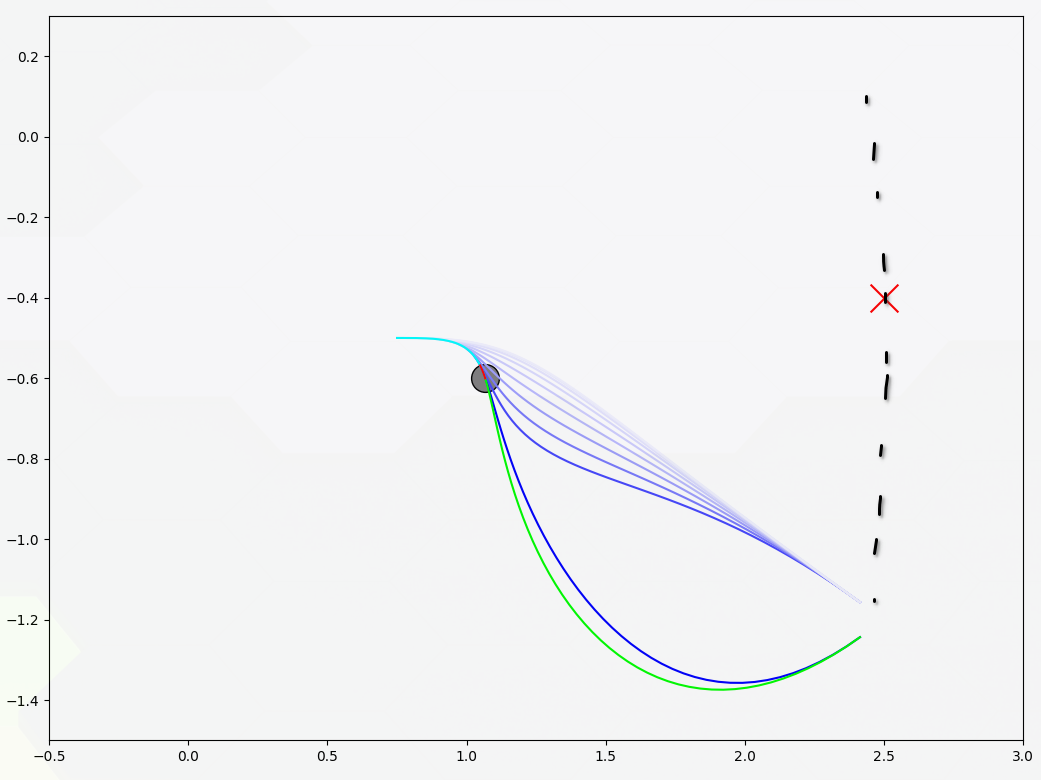
\includegraphics[width=0.8\textwidth]{trajectory-replanning}
    % This file was created with tikzplotlib v0.10.1.
\begin{tikzpicture}

\definecolor{cyan}{RGB}{0,255,255}
\definecolor{darkgray176}{RGB}{176,176,176}
\definecolor{gray}{RGB}{128,128,128}
\definecolor{lavender206206255}{RGB}{206,206,255}
\definecolor{lightsteelblue161161255}{RGB}{161,161,255}
\definecolor{lightsteelblue187187255}{RGB}{187,187,255}
\definecolor{mediumslateblue124124255}{RGB}{124,124,255}
\definecolor{royalblue7272255}{RGB}{72,72,255}

\begin{axis}[
width=0.8\textwidth,
xmin=0.5, xmax=3,
ymin=-1.5, ymax=-0.4,
axis equal,
legend entries={Traveled path,
                Previously planned Path, Currently planned Path, Start},
]
\addlegendimage{no markers,red, thick}
\addlegendimage{no markers,royalblue7272255, thick}
\addlegendimage{no markers, green, thick}
\addlegendimage{black, thick, mark=*, only marks}
\addplot [mark=*, black]
table {%
0.75 -0.5
}
\addplot [thick, blue]
table {%
0.936567748095716 -0.511242610456874
0.951437693831983 -0.516267025856055
0.965217950151147 -0.522419324901196
0.978131695001057 -0.529529211758212
0.990389039298842 -0.537441148536889
1.00218738690918 -0.546013874687306
1.01371179462259 -0.555119926396258
1.02513533213367 -0.564645155983677
1.03661944201944 -0.57448825129906
1.04831429971754 -0.584560255117888
1.06035917350456 -0.59478408453805
1.0728827844743 -0.605094050376269
1.08600366651606 -0.615435376564522
1.09983052629288 -0.625763719546462
1.11446260321984 -0.636044687673847
1.12999002944236 -0.646253360602955
1.14649418981442 -0.656373808691017
1.16404808187689 -0.666398612392629
1.18271667583578 -0.676328381656186
1.20255727454052 -0.686171275320296
1.22361987346221 -0.695942520510209
1.24594752067197 -0.70566393203424
1.26957667681913 -0.715363431780187
1.29453757510957 -0.725074568111761
1.32085458128394 -0.734836035265004
1.348546553596 -0.744691192744714
1.37762720279085 -0.754687584720869
1.40810545208322 -0.764876459425049
1.43998579713574 -0.775312288546861
1.47326866603723 -0.786052286630357
1.50795077928096 -0.797155930470465
1.54402550974295 -0.808684478509404
1.58148324266021 -0.820700490233116
1.62031173560905 -0.833267345567679
1.66049647848334 -0.84644876427574
1.70202105347279 -0.860308325352929
1.74486749504123 -0.874908986424293
1.78901664990487 -0.890312603140708
1.83444853701059 -0.906579448575308
1.88114270751422 -0.923767732619908
1.92907860475881 -0.941933121381427
1.9782359242529 -0.961128256578309
2.02859497364881 -0.98140227493695
2.08013703272091 -1.00280032758812
2.13284471334388 -1.02536309946337
2.18670231947101 -1.0491263286915
2.24169620711249 -1.07412032599493
2.29781514431362 -1.10036949408615
2.35505067113315 -1.12789184706413
2.41339745962156 -1.15669852981078
};
\addplot [thick, royalblue7272255]
table {%
0.903886181942021 -0.50486136545504
0.921859258398568 -0.507637363892377
0.93904078670725 -0.511177067131014
0.955566927124709 -0.515394128514011
0.971568342835892 -0.520210360314542
0.98717031310837 -0.525555460969289
1.00249284644664 -0.531366742311834
1.01765079374646 -0.537588856806062
1.03275396144911 -0.544173524779549
1.04790722469578 -0.551079261656959
1.06321064048181 -0.558271105193441
1.07875956081103 -0.565720342708023
1.09464474585009 -0.573404238317006
1.11095247708273 -0.581305760167361
1.12776467046415 -0.589413307670124
1.14515898957526 -0.597720438733787
1.16320895877702 -0.606225596997702
1.18198407636476 -0.614931839065465
1.20154992772249 -0.623846561738321
1.22196829847718 -0.632981229248553
1.24329728765312 -0.642351100492879
1.26559142082619 -0.651974956265848
1.28890176327821 -0.661874826493234
1.31327603315121 -0.672075717465431
1.33875871460177 -0.68260533907085
1.36539117095532 -0.693493832029311
1.39321175786048 -0.70477349512544
1.42225593644332 -0.716478512442067
1.4525563864617 -0.728644680593613
1.4841431194596 -0.741309135959494
1.5170435919214 -0.754510081917511
1.55128281842621 -0.768286516077249
1.58688348480218 -0.782677957513464
1.62386606128079 -0.797724173999491
1.6622489156512 -0.813464909240625
1.70204842641453 -0.829939610107528
1.74327909593818 -0.847187153869617
1.78595366361017 -0.865245575428462
1.83008321899339 -0.884151794551181
1.87567731497997 -0.903941343103831
1.92274408094558 -0.924648092284812
1.9712903359037 -0.946303979858254
2.02132170165998 -0.968938737387414
2.07284271596655 -0.992579617468075
2.1258569456763 -1.01725112096194
2.1803670998972 -1.04297472423001
2.23637514314664 -1.06976860636601
2.29388240850572 -1.09764737642978
2.35288971077354 -1.12662180068063
2.41339745962156 -1.15669852981078
};
\addplot [thick, mediumslateblue124124255]
table {%
0.86769790424018 -0.501736655416989
0.888040195200336 -0.50309730503939
0.907844272914256 -0.504940749732723
0.927176709503907 -0.507239655739161
0.946104618499477 -0.509970362138119
0.964695571263182 -0.513112747610113
0.983017513413069 -0.51665009720061
1.00113868124683 -0.520568969083892
1.01912751816559 -0.524859061326908
1.03705259109774 -0.529513078653133
1.05498250692271 -0.534526599206424
1.07298582889481 -0.539897941314878
1.09113099306701 -0.545628030254686
1.10948622471475 -0.551720265013993
1.12811945475974 -0.558180385056754
1.14709823619381 -0.565016337086588
1.16648966050264 -0.572238141810639
1.18636027408964 -0.579857760703429
1.20677599469969 -0.587888962770717
1.227802027843 -0.596347191313358
1.24950278321889 -0.605249430691152
1.2719417911396 -0.614614073086711
1.29518161895409 -0.624460785269306
1.31928378747186 -0.634810375358733
1.34430868738673 -0.645684659589161
1.37031549570069 -0.657106329072995
1.39736209214765 -0.669098816564732
1.42550497561728 -0.681686163224814
1.45479918057883 -0.694892885383489
1.48529819350489 -0.708743841304666
1.51705386929525 -0.72326409794977
1.55011634770064 -0.738478797741604
1.5845339697466 -0.754413025328201
1.62035319415724 -0.77109167434668
1.6576185137791 -0.788539314187108
1.69637237200487 -0.806780056756353
1.73665507919729 -0.825837423241942
1.77850472911288 -0.845734210875915
1.82195711532579 -0.866492359698688
1.8670456476516 -0.888132819322902
1.91380126857111 -0.910675415697288
1.96225236965415 -0.934138717870515
2.0124247079834 -0.958539904755054
2.06434132257819 -0.983894631891032
2.11802245081827 -1.01021689821009
2.1734854448677 -1.03751891279923
2.23074468809856 -1.0658109616647
2.28981151151482 -1.09510127449581
2.35069411017611 -1.12539589142881
2.41339745962156 -1.15669852981078
};
\addplot [thick, lightsteelblue161161255]
table {%
0.829383214992879 -0.500440812193034
0.851508477947783 -0.500988222670885
0.873298602348696 -0.50181376048788
0.894766674144783 -0.502928586126469
0.915930981444019 -0.504344753473229
0.936814778888565 -0.506075161281677
0.957446052030142 -0.508133504635102
0.977857281705406 -0.510534226409382
0.998085208411323 -0.513292468735806
1.01817059668054 -0.516424024463899
1.03815799945677 -0.519945288624245
1.05809552247014 -0.523873209891307
1.07803458861262 -0.528225242046248
1.09802970231331 -0.533019295439762
1.11813821391392 -0.538273688454883
1.13842008404406 -0.544007098969821
1.15893764799664 -0.550238515820777
1.17975538010328 -0.556987190264764
1.20093965810962 -0.564272587442435
1.22255852755075 -0.572114337840903
1.24468146612656 -0.580532188756562
1.26737914807711 -0.589545955757912
1.29072320855803 -0.59917547414838
1.31478600801585 -0.609440550429142
1.33964039656343 -0.620360913761947
1.36535947835529 -0.631956167431938
1.392016375963 -0.644245740310476
1.41968399475056 -0.657248838317962
1.44843478724976 -0.670984395886657
1.47834051753559 -0.685471027423508
1.50947202560155 -0.700726978772971
1.54189899173509 -0.716770078679829
1.57568970089295 -0.733617690252017
1.61091080707654 -0.751286662423445
1.64762709770733 -0.769793281416822
1.68590125800219 -0.789153222206473
1.72579363534879 -0.809381499981169
1.767362003681 -0.83049242160694
1.81066132785418 -0.852499537089909
1.85574352802066 -0.875415591039104
1.90265724400503 -0.899252474129286
1.95144759967958 -0.924021174563772
2.0021559673396 -0.949731729537253
2.05481973207884 -0.976393176698622
2.10947205616481 -1.00401350561379
2.1661416434142 -1.03259960922852
2.22485250356824 -1.06215723533123
2.28562371666809 -1.09269093801584
2.34846919743016 -1.12420402914457
2.41339745962156 -1.15669852981078
};
\addplot [thick, lightsteelblue187187255]
table {%
0.789926649360842 -0.500049598310148
0.813389027593452 -0.500195024727243
0.836671446570459 -0.500477624725688
0.859747200438726 -0.500931217145072
0.882598296136937 -0.501589031907685
0.905215102794054 -0.502483704725086
0.927596001127766 -0.503647271804675
0.949747032842946 -0.505111164556269
0.9716815500301 -0.506906204298669
0.993419864563821 -0.509062596966236
1.01498889750125 -0.511609927815461
1.0364218284805 -0.514577156131537
1.05775774511915 -0.517992609934935
1.07904129241269 -0.521883980687969
1.10032232213291 -0.526278318001374
1.12165554222647 -0.531202024340877
1.14310016621323 -0.536680849733767
1.16471956258481 -0.542739886475468
1.18658090420294 -0.549403563836115
1.20875481769801 -0.556695642767117
1.23131503286747 -0.56463921060774
1.25433803207426 -0.573256675791672
1.27790269964534 -0.582569762553595
1.30208997127006 -0.592599505635762
1.32698248339867 -0.603366244994566
1.35266422264075 -0.61488962050711
1.37922017516366 -0.627188566677783
1.40673597609099 -0.640281307344832
1.43529755890105 -0.65418535038693
1.46499080482526 -0.668917482429752
1.49590119224666 -0.684493763552546
1.52811344609834 -0.700929521994706
1.56171118726187 -0.71823934886234
1.59677658196579 -0.736437092834849
1.63338999118406 -0.755535854871492
1.67162962003448 -0.775547982917965
1.71157116717717 -0.796485066612965
1.75328747421302 -0.818357931994772
1.79684817508215 -0.841176636207812
1.84231934546232 -0.864950462209234
1.88976315216745 -0.889687913475481
1.93923750254601 -0.915396708708862
1.99079569387953 -0.942083776544124
2.04448606278099 -0.969755250255027
2.10035163459334 -0.998416462460908
2.15842977278789 -1.02807193983326
2.21875182836281 -1.05872539780232
2.28134278924156 -1.09037973526359
2.34622092967134 -1.12303702928446
2.41339745962156 -1.15669852981078
};
\addplot [thick, lavender206206255]
table {%
0.75 -0.5
0.774474001881514 -0.500007724820588
0.79888172961365 -0.500061415533454
0.823167646041292 -0.500205988410129
0.847287530291339 -0.500485222186761
0.871208041289807 -0.500941766320088
0.894906281278931 -0.50161714924341
0.918369359334266 -0.502551786622568
0.941593954881789 -0.503784989611914
0.964585881214997 -0.505354973110284
0.987359649012017 -0.507298864016975
1.0099380298527 -0.509652709487717
1.03235161973571 -0.51245148519065
1.05463840259568 -0.515729103562293
1.07684331382022 -0.519518422063519
1.09901780376712 -0.523851251435535
1.12121940128138 -0.528758363955847
1.14351127721233 -0.534269501694239
1.16596180793076 -0.540413384768749
1.18864413884598 -0.547217719601635
1.21163574792294 -0.554709207175358
1.23501800919934 -0.56291355128855
1.25887575630272 -0.571855466811989
1.28329684596758 -0.581558687944577
1.30837172155243 -0.592045976469306
1.33419297655696 -0.603339130009241
1.36085491813909 -0.615458990283485
1.38845313063211 -0.62842545136316
1.41708403906175 -0.642257467927378
1.4468444726633 -0.656973063519216
1.47783122839869 -0.672589338801686
1.51014063447364 -0.689122479813714
1.54386811385468 -0.706587766226114
1.57910774778635 -0.724999579597555
1.61595183930822 -0.744371411630545
1.65449047677205 -0.764715872427394
1.69481109735882 -0.7860446987462
1.73699805059593 -0.808368762256811
1.78113216187422 -0.831698077796807
1.82729029596509 -0.856041811627471
1.87554492053763 -0.881408289689763
1.9259636696757 -0.907805005860296
1.97860890739503 -0.935238630207304
2.03353729116033 -0.963715017246624
2.09079933540238 -0.993239214197664
2.15043897503514 -1.02381546923938
2.21249312897286 -1.05544723976625
2.27699126364717 -1.08813720064423
2.34395495652417 -1.12188725246678
2.41339745962155 -1.15669852981078
};
\addplot [thick, green]
table {%
0.963899676615637 -0.522968099013425
0.974803630308841 -0.531377935858995
0.984293087538302 -0.541649012948189
0.992694822355425 -0.553756391693564
1.00031344834871 -0.567663857711007
1.00743207596587 -0.583324428439328
1.01431296983592 -0.600680860759844
1.02119820609129 -0.619666158615968
1.02831032968993 -0.640204080632795
1.03585301173744 -0.662209647736688
1.04401170680915 -0.68558965077487
1.05295431027221 -0.710243158135003
1.06283181560776 -0.736062023364784
1.07377897173297 -0.762931392791525
1.0859149403232 -0.790730213141745
1.09934395313405 -0.819331739160753
1.11415596932352 -0.848604041232241
1.13042733277411 -0.878410512997863
1.14822142941487 -0.90861037897683
1.16758934454359 -0.939059202185493
1.18857052014885 -0.969609391756929
1.21119341223214 -1.00011071056053
1.23547614812998 -1.0304107828216
1.261427183836 -1.06035560174091
1.28904596132309 -1.08979003711434
1.31832356586546 -1.11855834295239
1.34924338336077 -1.14650466509986
1.38178175765224 -1.17347354885535
1.41590864785076 -1.1993104465909
1.45158828565696 -1.22386222537156
1.48877983268338 -1.24697767457498
1.52743803777651 -1.26850801351099
1.56751389433896 -1.28830739904122
1.6089552976515 -1.30623343319862
1.65170770219524 -1.32214767080711
1.69571477897368 -1.33591612710115
1.74091907283482 -1.34740978534531
1.78726265979332 -1.35650510445388
1.83468780435254 -1.36308452661043
1.88313761682669 -1.36703698488743
1.93255671066293 -1.36825841086582
1.98289185976345 -1.36665224225457
2.03409265580762 -1.36212993051035
2.08611216557406 -1.354611448457
2.13890758826276 -1.34402579790522
2.19244091281721 -1.3303115172721
2.24667957524644 -1.31341718920073
2.30159711594723 -1.29330194817978
2.35717383702611 -1.26993598816308
2.41339745962155 -1.24330107018922
};
\addplot [thick, mumred]
table {%
0.75 -0.5
0.750199999132093 -0.50000000055881
0.750199999132093 -0.50000000055881
0.750399997398152 -0.500000001675222
0.75059999480005 -0.500000003348033
0.750799991339652 -0.500000005576041
0.750999987018822 -0.500000008358045
0.751199981839417 -0.500000011692851
0.751399975803292 -0.500000015579263
% 0.751599968912297 -0.50000002001609
% 0.75179996116828 -0.500000025002143
% 0.751999952573082 -0.500000030536237
% 0.752199943128543 -0.500000036617186
% 0.752399932836497 -0.500000043243811
% 0.752599921698774 -0.500000050414932
% 0.7527999097172 -0.500000058129373
% 0.7529998968936 -0.50000006638596
% 0.753199883229792 -0.500000075183523
% 0.753399868727589 -0.500000084520893
% 0.753599853388804 -0.500000094396905
% 0.753799837215244 -0.500000104810393
% 0.753999820208711 -0.500000115760199
% 0.754199801423924 -0.500000127867992
% 0.754399780864724 -0.500000141131271
% 0.754599758534945 -0.500000155547541
% 0.754799734438409 -0.50000017111431
% 0.754999708578935 -0.500000187829094
% 0.755199680960328 -0.500000205689413
% 0.75539965158639 -0.500000224692793
% 0.755599620460912 -0.500000244836765
% 0.755799587587677 -0.500000266118865
% 0.75599955297046 -0.500000288536634
% 0.756199516613029 -0.50000031208762
% 0.756399478519141 -0.500000336769375
% 0.756599438692549 -0.500000362579456
% 0.756799397136994 -0.500000389515427
% 0.756999353856211 -0.500000417574855
% 0.757199308853926 -0.500000446755313
% 0.757399262133859 -0.500000477054381
% 0.757599213699719 -0.500000508469642
% 0.757799163555209 -0.500000540998685
% 0.757999111704023 -0.500000574639104
% 0.758199057120232 -0.500000610078972
% 0.758398999809738 -0.500000647314402
% 0.758598939778431 -0.500000686341515
% 0.758798877032187 -0.500000727156442
% 0.758998811576872 -0.50000076975532
% 0.759198743418336 -0.500000814134297
% 0.759398672562419 -0.500000860289528
% 0.759598599014947 -0.500000908217175
% 0.759798522781734 -0.50000095791341
% 0.75999844386858 -0.500001009374414
% 0.760198362281276 -0.500001062596374
% 0.760398278025595 -0.500001117575486
% 0.760598191107304 -0.500001174307956
0.760798101532152 -0.500001232789995
0.760998009305878 -0.500001293017825
0.76119791443421 -0.500001354987676
0.76139781692286 -0.500001418695783
0.761597716777532 -0.500001484138393
% 0.761797614003913 -0.500001551311759
% 0.761997508607681 -0.500001620212142
% 0.762197399478882 -0.500001691597702
% 0.762397286625579 -0.500001765463071
% 0.762597170055815 -0.500001841802892
% 0.762797049777619 -0.500001920611821
% 0.762996925799 -0.500002001884524
% 0.763196798127953 -0.500002085615679
% 0.763396666772451 -0.500002171799977
% 0.763596531740455 -0.500002260432118
% 0.763796393039904 -0.500002351506815
% 0.763996250678724 -0.500002445018793
% 0.76419610466482 -0.500002540962786
% 0.764395955006083 -0.500002639333541
% 0.764595801710387 -0.500002740125818
% 0.764795644785585 -0.500002843334384
% 0.764995484239518 -0.500002948954022
% 0.765195320080008 -0.500003056979522
% 0.765395152314859 -0.500003167405689
% 0.76559498095186 -0.500003280227338
% 0.765794805998781 -0.500003395439292
% 0.765994627463378 -0.500003513036391
% 0.76619444414819 -0.500003633850713
% 0.766394256063542 -0.500003757875308
% 0.766594063219736 -0.500003885103243
% 0.76679386562705 -0.500004015527598
% 0.766993663295744 -0.50000414914147
% 0.767193456236052 -0.500004285937968
% 0.767393244458188 -0.500004425910219
% 0.767593027972342 -0.500004569051362
% 0.767792806788685 -0.500004715354553
% 0.767992580917363 -0.500004864812962
% 0.768192350368502 -0.500005017419774
% 0.768392115152206 -0.500005173168187
% 0.768591875278555 -0.500005332051417
% 0.76879163075761 -0.500005494062691
% 0.768991381599409 -0.500005659195254
% 0.769191127813969 -0.500005827442364
% 0.769390869411283 -0.500005998797292
% 0.769590606401327 -0.500006173253327
% 0.76979033879405 -0.500006350803769
% 0.769990066599384 -0.500006531441935
% 0.770189788528776 -0.500006716077809
% 0.770389504594918 -0.500006904702758
% 0.770589214810475 -0.500007097308164
% 0.770788919188083 -0.50000729388543
% 0.770988617740353 -0.500007494425976
% 0.771188310479868 -0.500007698921242
% 0.771387997419183 -0.500007907362686
% 0.771587678570827 -0.500008119741783
% 0.7717873539473 -0.500008336050029
0.771987023561078 -0.500008556278937
0.772186687424607 -0.500008780420037
0.772386345550309 -0.500009008464881
0.772585997950577 -0.500009240405034
% 0.772785644637777 -0.500009476232084
% 0.772985285624251 -0.500009715937635
% 0.773184920922312 -0.50000995951331
% 0.773384550544246 -0.500010206950748
% 0.773584174502314 -0.500010458241609
% 0.77378379280875 -0.500010713377569
% 0.773983405475762 -0.500010972350322
% 0.774183011120011 -0.500011236151902
% 0.774382609756668 -0.500011504771879
% 0.774582201400868 -0.500011778199845
% 0.774781786067715 -0.500012056425414
% 0.77498136377228 -0.500012339438223
% 0.775180934529602 -0.500012627227933
% 0.775380498354686 -0.500012919784225
% 0.775580055262507 -0.500013217096803
% 0.775779605268006 -0.500013519155393
% 0.775979148386091 -0.500013825949745
% 0.77617868463164 -0.50001413746963
% 0.776378214019497 -0.500014453704839
% 0.776577736564474 -0.500014774645187
% 0.776777252281353 -0.500015100280513
% 0.776976761184882 -0.500015430600674
% 0.777176263289779 -0.500015765595551
% 0.777375758610726 -0.500016105255048
% 0.77757524716238 -0.500016449569087
% 0.77777472895936 -0.500016798527616
% 0.777974204016257 -0.500017152120603
% 0.778173670851148 -0.50001751142643
% 0.778373129481791 -0.500017876432758
% 0.778572579925907 -0.500018247127274
% 0.77877202220118 -0.500018623497691
% 0.778971456325254 -0.50001900553175
% 0.779170882315737 -0.500019393217216
% 0.779370300190195 -0.500019786541884
% 0.779569709966161 -0.500020185493571
% 0.779769111661126 -0.500020590060124
% 0.779968505292547 -0.500021000229415
% 0.780167890877839 -0.500021415989342
% 0.780367268434383 -0.500021837327829
% 0.78056663797952 -0.500022264232826
% 0.780765999530556 -0.50002269669231
% 0.780965353104758 -0.500023134694282
% 0.781164698719355 -0.500023578226772
% 0.78136403639154 -0.500024027277833
% 0.78156336613847 -0.500024481835546
% 0.781762687977262 -0.500024941888015
% 0.781962001924998 -0.500025407423372
% 0.782161306397257 -0.500025879610817
0.782360601414507 -0.500026358435982
0.782559886997171 -0.500026843884528
0.782759163165627 -0.50002733594215
0.782958429940209 -0.500027834594572
0.783157687341209 -0.500028339827548
0.783356935388874 -0.500028851626866
0.783556174103406 -0.500029369978341
0.783755403504966 -0.500029894867821
0.783954623613669 -0.500030426281185
0.784153834449588 -0.500030964204339
0.784353036032752 -0.500031508623224
% 0.784552228383147 -0.500032059523809
% 0.784751411520716 -0.500032616892092
% 0.784950585465358 -0.500033180714104
% 0.785149750236931 -0.500033750975905
% 0.785348905855248 -0.500034327663584
% 0.78554805234008 -0.500034910763263
% 0.785747189711155 -0.50003550026109
% 0.78594631798816 -0.500036096143246
% 0.786145435480157 -0.500036699674382
% 0.786344542210442 -0.500037310837976
% 0.786543638202259 -0.500037929617541
% 0.786742723478806 -0.500038555996628
% 0.786941798063225 -0.500039189958822
% 0.787140861978613 -0.500039831487742
% 0.787339915248014 -0.500040480567045
% 0.787538957894424 -0.500041137180421
% 0.787737989940788 -0.500041801311598
% 0.787937011410002 -0.500042472944337
% 0.788136022324914 -0.500043152062434
% 0.78833502270832 -0.500043838649722
% 0.788534012582969 -0.500044532690066
% 0.788732991971559 -0.500045234167367
% 0.78893196089674 -0.500045943065564
% 0.789130919381113 -0.500046659368625
% 0.789329867447231 -0.500047383060557
% 0.789528805117596 -0.500048114125399
% 0.789727732414665 -0.500048852547226
% 0.789926649360842 -0.500049598310148
% 0.790125554154544 -0.500050352779072
% 0.790125554154544 -0.500050352779072
% 0.79032444682202 -0.500051115935192
% 0.790523327389463 -0.500051887759746
% 0.790722195883009 -0.500052668234009
% 0.790921052328738 -0.500053457339297
% 0.791119896752673 -0.500054255056969
% 0.791318729180781 -0.50005506136842
% 0.791517549638972 -0.500055876255088
% 0.791716358153103 -0.500056699698451
% 0.791915154748972 -0.500057531680027
% 0.792113939452322 -0.500058372181373
% 0.792312712288842 -0.500059221184086
% 0.792511473284164 -0.500060078669803
% 0.792710222463864 -0.500060944620201
% 0.792908959853465 -0.500061819016996
% 0.793107685478433 -0.500062701841944
% 0.79330639936418 -0.50006359307684
% 0.793505101536063 -0.50006449270352
% 0.793703792019382 -0.500065400703855
% 0.793902470839387 -0.50006631705976
% 0.794101136079603 -0.500067243241382
% 0.794299787769363 -0.500068179227497
% 0.794498425937936 -0.500069124996928
% 0.794697050614527 -0.500070080528543
% 0.79489566182828 -0.500071045801255
% 0.795094259608274 -0.500072020794023
% 0.795292843983526 -0.500073005485853
% 0.795491414982991 -0.500073999855794
% 0.795689972635559 -0.500075003882942
% 0.79588851697006 -0.500076017546436
% 0.796087048015262 -0.500077040825464
% 0.796285565799869 -0.500078073699254
% 0.796484070352524 -0.500079116147082
% 0.796682561701808 -0.500080168148269
% 0.79688103987624 -0.500081229682179
0.797079504904279 -0.500082300728221
0.79727795681432 -0.50008338126585
0.797476395634697 -0.500084471274563
0.797674821393686 -0.500085570733902
0.797873234119498 -0.500086679623455
0.798071631776417 -0.50008779952377
0.798270014396993 -0.500088930411064
0.798468382013703 -0.500090072261604
0.798666734658956 -0.50009122505171
0.798865072365091 -0.500092388757752
0.799063395164376 -0.500093563356153
% 0.799261703089009 -0.500094748823384
% 0.799459996171121 -0.500095945135969
% 0.79965827444277 -0.500097152270482
% 0.799856537935947 -0.500098370203548
% 0.800054786682575 -0.500099598911841
% 0.800253020714505 -0.500100838372088
% 0.800451240063521 -0.500102088561064
% 0.800649444761339 -0.500103349455594
% 0.800847634839604 -0.500104621032556
% 0.801045810329895 -0.500105903268874
% 0.801243971263723 -0.500107196141526
% 0.801442117672529 -0.500108499627535
% 0.801640249587687 -0.500109813703978
% 0.801838367040503 -0.500111138347979
% 0.802036467871553 -0.500112475255831
% 0.80223455211674 -0.500113824401045
% 0.80243261981189 -0.500115185757187
% 0.80263067099275 -0.500116559297882
% 0.802828705694992 -0.500117944996812
% 0.803026723954208 -0.500119342827714
% 0.803224725805917 -0.500120752764383
% 0.803422711285559 -0.500122174780672
% 0.803620680428496 -0.500123608850488
% 0.803818633270017 -0.500125054947795
% 0.804016569845332 -0.500126513046615
% 0.804214490189576 -0.500127983121023
% 0.804412394337809 -0.500129465145153
% 0.804610282325014 -0.500130959093193
% 0.804808154186098 -0.500132464939387
% 0.805006009955894 -0.500133982658037
% 0.80520384966916 -0.500135512223496
% 0.805401673360577 -0.500137053610176
% 0.805599481064753 -0.500138606792543
% 0.80579727281622 -0.500140171745118
% 0.805995046327267 -0.500141750285471
% 0.806192801637294 -0.500143342384251
0.806390538785615 -0.500144948012173
0.80658825781146 -0.500146567140013
0.806785958753972 -0.500148199738612
0.806983641652212 -0.500149845778873
0.807181306545155 -0.500151505231761
0.807378953471693 -0.500153178068307
0.807576582470634 -0.5001548642596
0.8077741935807 -0.500156563776795
0.807971786840533 -0.500158276591107
0.808169362288688 -0.500160002673815
0.808366919963638 -0.50016174199626
0.808564459903774 -0.500163494529843
0.808761982147403 -0.500165260246028
0.80895948673275 -0.500167039116341
0.809156973697956 -0.500168831112369
% 0.80935444308108 -0.50017063620576
% 0.809551894920101 -0.500172454368224
% 0.809749329252913 -0.500174285571533
% 0.809946743658831 -0.50017613176025
% 0.810144138180896 -0.500177992902008
% 0.810341512862057 -0.500179868964507
% 0.810538867745172 -0.50018175991552
% 0.810736202873003 -0.500183665722887
% 0.810933518288223 -0.500185586354517
% 0.81113081403341 -0.500187521778392
% 0.811328090151052 -0.500189471962559
% 0.811525346683544 -0.500191436875136
% 0.81172258367319 -0.50019341648431
% 0.811919801162202 -0.500195410758337
% 0.812116999192703 -0.500197419665539
% 0.812314177806722 -0.50019944317431
% 0.812511337046199 -0.500201481253111
% 0.812708476952984 -0.500203533870469
% 0.812905597568833 -0.500205600994982
% 0.813102698935417 -0.500207682595314
% 0.813299781094314 -0.500209778640197
% 0.813496844087011 -0.500211889098431
% 0.813693887954909 -0.500214013938884
% 0.813890910139545 -0.50021615523903
% 0.814087910687754 -0.500218312963315
% 0.814284889646273 -0.500220487076265
% 0.814481847061734 -0.500222677542479
% 0.814678782980671 -0.500224884326634
% 0.814875697449516 -0.500227107393484
% 0.815072590514601 -0.500229346707858
% 0.815269462222158 -0.500231602234662
% 0.81546631261832 -0.500233873938876
% 0.815663141749119 -0.500236161785557
% 0.815859949660489 -0.500238465739837
0.816056736398263 -0.500240785766925
0.816253502008176 -0.500243121832103
0.816450246535865 -0.500245473900728
0.816646970026866 -0.500247841938233
0.81684367252662 -0.500250225910126
0.817040354080468 -0.500252625781988
0.817237014733652 -0.500255041519475
0.817433654531318 -0.500257473088317
0.817630273518515 -0.500259920454319
% 0.817826868994092 -0.500262385833975
% 0.818023441008836 -0.500264869188375
% 0.818219989613422 -0.500267370478694
% 0.818416514858415 -0.500269889666189
% 0.818613016794273 -0.500272426712204
% 0.818809495471343 -0.500274981578164
% 0.819005950939864 -0.500277554225577
% 0.819202383249967 -0.500280144616037
% 0.819398792451673 -0.500282752711217
% 0.819595178594897 -0.500285378472875
% 0.819791541729446 -0.500288021862853
% 0.819987881905018 -0.500290682843073
% 0.820184199171204 -0.500293361375539
% 0.820380493577489 -0.50029605742234
% 0.82057676517325 -0.500298770945643
% 0.820773014007757 -0.500301501907701
% 0.820969240130176 -0.500304250270845
% 0.821165443589564 -0.500307015997488
% 0.821361624434873 -0.500309799050127
% 0.82155778271495 -0.500312599391335
% 0.821753915580939 -0.500315419382936
% 0.821950023087734 -0.500318258982485
% 0.822146105290111 -0.500321118147627
% 0.822342162242727 -0.500323996836103
% 0.822538194000123 -0.50032689500574
% 0.82273420061672 -0.500329812614461
0.822930182146821 -0.500332749620276
0.823126138644614 -0.500335705981287
0.823322070164169 -0.500338681655688
0.823517976759438 -0.500341676601762
0.823713858484259 -0.500344690777881
0.82390971539235 -0.50034772414251
0.824105547537317 -0.5003507766542
0.824301354972647 -0.500353848271594
0.824497137751714 -0.500356938953424
0.824692895927775 -0.50036004865851
0.824888629553972 -0.500363177345763
0.825084338683333 -0.50036632497418
% 0.825280023368772 -0.50036949150285
% 0.825475683663087 -0.500372676890946
% 0.825671316564586 -0.50037588365213
% 0.825866922132438 -0.500379111740236
% 0.826062500425684 -0.500382361109196
% 0.826258051503237 -0.500385631713045
% 0.826453575423882 -0.500388923505915
% 0.826649072246279 -0.500392236442037
% 0.82684454202896 -0.500395570475744
% 0.82703998483033 -0.500398925561462
% 0.82723540070867 -0.500402301653722
% 0.827430789722132 -0.500405698707147
% 0.827626151928746 -0.500409116676462
% 0.827821487386413 -0.500412555516489
% 0.828016796152912 -0.500416015182147
% 0.828212078285896 -0.500419495628453
% 0.828407333842892 -0.50042299681052
% 0.828602562881306 -0.500426518683559
% 0.828797765458417 -0.500430061202878
% 0.828992941631381 -0.50043362432388
% 0.829188091457232 -0.500437208002067
% 0.829383214992879 -0.500440812193034
% 0.829578309078561 -0.500444439568994
% 0.829578309078561 -0.500444439568994
% 0.829773373777888 -0.500448090079866
% 0.829968409154335 -0.500451763675681
% 0.83016341527124 -0.500455460306573
% 0.830358392191803 -0.500459179922788
% 0.830553339979089 -0.500462922474677
0.830748258696025 -0.500466687912699
0.830943148405404 -0.50047047618742
0.831138009169881 -0.500474287249512
0.831332841051977 -0.500478121049756
0.831527644114079 -0.500481977539036
0.831722418418438 -0.500485856668345
0.831917164027171 -0.500489758388779
0.832111881002259 -0.500493682651542
0.832306569405552 -0.500497629407942
0.832501229298765 -0.500501598609394
% 0.832695860743479 -0.500505590207416
% 0.832890463801143 -0.500509604153631
% 0.833085038533074 -0.500513640399768
% 0.833279585000455 -0.500517698897658
% 0.833474099880113 -0.500521782484986
% 0.833668583240278 -0.500525891107559
% 0.833863035149032 -0.500530024711302
% 0.83405745567431 -0.500534183242254
% 0.8342518448839 -0.500538366646573
% 0.834446202845444 -0.500542574870532
% 0.834640529626438 -0.500546807860522
% 0.834834825294233 -0.500551065563046
% 0.835029089916031 -0.500555347924728
% 0.835223323558894 -0.500559654892301
% 0.835417526289735 -0.500563986412619
% 0.835611698175324 -0.500568342432646
% 0.835805839282287 -0.500572722899464
% 0.835999949677106 -0.500577127760267
% 0.836194029426119 -0.500581556962365
% 0.836388078595521 -0.50058601045318
% 0.836582097251364 -0.500590488180249
0.836776085459558 -0.500594990091221
0.836970043285868 -0.500599516133859
0.837163970795921 -0.500604066256038
0.837357864497692 -0.500608643468046
0.837551724464207 -0.500613247711368
0.837745550768334 -0.500617878927617
0.837939343482784 -0.500622537058531
0.83813310268011 -0.500627222045974
0.83832682843271 -0.500631933831936
0.838520520812825 -0.500636672358532
% 0.838714179892538 -0.500641437568004
% 0.838907805743779 -0.500646229402715
% 0.839101398438321 -0.500651047805155
% 0.839294958047783 -0.500655892717937
% 0.839488484643628 -0.500660764083801
% 0.839681978297166 -0.500665661845606
% 0.839875439079552 -0.500670585946338
% 0.840068867061788 -0.500675536329104
% 0.840262262314723 -0.500680512937136
% 0.840455624909051 -0.500685515713786
% 0.840648954915315 -0.500690544602531
% 0.840842252403905 -0.500695599546969
% 0.84103551744506 -0.500700680490818
% 0.841228746372363 -0.500705790624307
% 0.841421939263821 -0.500710929884384
% 0.841615096197271 -0.500716098208138
% 0.841808217250382 -0.50072129553279
% 0.842001302500656 -0.500726521795698
% 0.842194352025427 -0.500731776934356
% 0.842387365901862 -0.500737060886392
% 0.842580344206962 -0.50074237358957
% 0.84277328701756 -0.500747714981786
0.842966194410324 -0.500753085001073
0.843159066461758 -0.500758483585595
0.843351903248198 -0.500763910673653
0.843544704845817 -0.500769366203678
0.843737471330623 -0.500774850114236
0.843930202778459 -0.500780362344024
0.844122899265005 -0.500785902831874
0.844315560865778 -0.500791471516748
0.84450818765613 -0.50079706833774
0.844700779711253 -0.500802693234076
0.844893337106175 -0.500808346145114
0.84508585599445 -0.500814030448571
0.845278336459254 -0.500819746076638
0.845470778583581 -0.500825492961654
% 0.845663182450247 -0.500831271036106
% 0.845855548141888 -0.500837080232622
% 0.846047875740962 -0.500842920483981
% 0.846240165329749 -0.500848791723102
% 0.846432416990352 -0.500854693883054
% 0.846624630804694 -0.500860626897046
% 0.846816806854525 -0.500866590698434
% 0.847008945221416 -0.500872585220718
% 0.847201045986761 -0.500878610397539
% 0.84739310923178 -0.500884666162685
% 0.847585135037516 -0.500890752450084
% 0.84777712348484 -0.500896869193809
% 0.847969074654445 -0.500903016328073
% 0.84816098862685 -0.500909193787234
% 0.848352865482402 -0.500915401505789
% 0.848544705301273 -0.500921639418378
% 0.848736508163463 -0.500927907459782
% 0.848928270036769 -0.50093420920297
% 0.849119991009728 -0.500940544575146
% 0.849311671170684 -0.500946913503672
% 0.849503310607791 -0.500953315916064
% 0.849694909409014 -0.50095975174
% 0.849886467662124 -0.500966220903308
% 0.850077985454707 -0.500972723333978
% 0.850269462874157 -0.50097925896015
% 0.850460900007679 -0.500985827710123
% 0.850652296942293 -0.500992429512349
% 0.850843653764826 -0.500999064295435
% 0.851034970561922 -0.501005731988144
% 0.851226247420035 -0.501012432519389
0.851417484425433 -0.50101916581824
0.851608681664199 -0.501025931813918
0.851799839222227 -0.501032730435799
0.85199095718523 -0.50103956161341
0.852182035638731 -0.501046425276431
0.852373074668072 -0.501053321354693
0.852564074358408 -0.501060249778179
0.852755030485964 -0.501067214323084
0.852945943144834 -0.501074214911386
0.853136812428912 -0.501081251465232
0.853327638431887 -0.501088323906935
% 0.853518421247246 -0.501095432158978
% 0.853709160968274 -0.501102576144011
% 0.853899857688055 -0.50110975578485
% 0.854090511499472 -0.501116971004479
% 0.854281122495206 -0.501124221726048
% 0.854471690767741 -0.501131507872872
% 0.854662216409357 -0.501138829368433
% 0.854852699512138 -0.501146186136378
% 0.855043140167967 -0.501153578100518
% 0.85523353846853 -0.501161005184829
% 0.855423894505314 -0.501168467313453
% 0.85561420836961 -0.501175964410692
% 0.855804480152509 -0.501183496401016
% 0.855994709944907 -0.501191063209054
% 0.856184897837504 -0.501198664759601
% 0.856375043920804 -0.501206300977613
% 0.856565143773555 -0.501213975850699
% 0.856755197495614 -0.501221689295364
% 0.856945205186626 -0.501229441228292
% 0.857135166946015 -0.50123723156635
% 0.857325082872995 -0.501245060226583
% 0.857514953066564 -0.501252927126214
% 0.857704777625506 -0.501260832182646
% 0.857894556648392 -0.501268775313461
% 0.858084290233579 -0.501276756436418
% 0.858273978479213 -0.501284775469454
% 0.858463621483228 -0.501292832330683
% 0.858653219343344 -0.501300926938397
% 0.858842772157074 -0.501309059211063
% 0.859032280021718 -0.501317229067324
% 0.859221743034364 -0.501325436426
% 0.859411161291895 -0.501333681206086
% 0.85960053489098 -0.501341963326752
0.859789863928082 -0.501350282707342
0.859979148499455 -0.501358639267374
0.860168388701145 -0.501367032926541
0.860357579908446 -0.501375467892265
0.860546722227186 -0.501383944075325
0.860735815762964 -0.501392461386689
0.860924860621152 -0.501401019737523
0.861113856906893 -0.501409619039179
0.861302804725104 -0.501418259203205
0.861491704180474 -0.501426940141337
% 0.861680555377467 -0.501435661765504
% 0.861869358420322 -0.501444423987824
% 0.862058113413051 -0.501453226720605
% 0.862246820459442 -0.501462069876344
% 0.862435479663061 -0.501470953367727
% 0.862624091127246 -0.50147987710763
% 0.862812654955115 -0.501488841009115
% 0.863001171249563 -0.501497844985435
% 0.863189640113262 -0.501506888950026
% 0.863378061648662 -0.501515972816515
% 0.863566435957993 -0.501525096498713
% 0.863754763143262 -0.501534259910619
% 0.863943043306258 -0.501543462966416
% 0.864131271612768 -0.501552710101951
% 0.864319448174804 -0.501562001222012
% 0.864507573104133 -0.501571336231593
% 0.864695646512281 -0.501580715035891
% 0.864883668510535 -0.501590137540312
% 0.86507163920994 -0.501599603650461
% 0.865259558721301 -0.501609113272151
% 0.865447427155185 -0.501618666311397
% 0.865635244621918 -0.501628262674417
% 0.86582301123159 -0.501637902267632
% 0.866010727094053 -0.501647584997664
% 0.866198392318919 -0.501657310771338
% 0.866386007015567 -0.501667079495679
0.866573571293138 -0.501676891077915
0.866761085260535 -0.501686745425472
0.86694854902643 -0.501696642445977
0.867135962699258 -0.501706582047256
0.86732332638722 -0.501716564137336
0.867510640198282 -0.501726588624439
0.86769790424018 -0.501736655416989
0.867885113463077 -0.50174676918808
0.867885113463077 -0.50174676918808
% 0.868072267985382 -0.501756929836236
% 0.868259367925249 -0.501767137260205
% 0.868446413400575 -0.501777391358949
% 0.868633404529005 -0.501787692031653
% 0.868820341427926 -0.501798039177715
% 0.869007224214476 -0.501808432696753
% 0.869194053005537 -0.501818872488603
% 0.869380827917738 -0.501829358453314
% 0.869567549067459 -0.501839890491153
% 0.869754216570826 -0.501850468502602
% 0.869940830543716 -0.501861092388359
% 0.870127391101754 -0.501871762049334
% 0.870313898360316 -0.501882477386653
% 0.87050035243453 -0.501893238301656
% 0.870686753439273 -0.501904044695895
% 0.870873101489175 -0.501914896471133
% 0.87105939669862 -0.501925793529349
% 0.871245639181741 -0.501936735772732
% 0.871431829052429 -0.50194772310368
% 0.871617961039045 -0.501958760441565
% 0.87180403526662 -0.50196984767837
% 0.871990051859911 -0.501980984706316
% 0.872176010943411 -0.501992171417851
% 0.872361912641339 -0.502003407705661
% 0.872547757077648 -0.50201469346266
% 0.872733544376024 -0.502026028581996
% 0.872919274659885 -0.502037412957044
% 0.873104948052381 -0.502048846481413
0.873290564676399 -0.50206032904894
0.873476124654558 -0.502071860553693
0.873661628109213 -0.502083440889966
0.873847075162456 -0.502095069952284
0.874032465936112 -0.502106747635398
0.874217800551746 -0.502118473834288
0.87440307913066 -0.502130248444159
0.874588301793892 -0.502142071360443
0.87477346866222 -0.5021539424788
0.874958579856162 -0.502165861695112
0.875143635495975 -0.502177828905487
0.875328630081988 -0.502189849284809
0.875513563746078 -0.502201922718232
0.875698436619836 -0.502214049091159
0.87588324883457 -0.502226228289241
0.876068000521303 -0.502238460198375
0.876252691810776 -0.502250744704707
0.876437322833446 -0.502263081694625
0.87662189371949 -0.502275471054765
0.876806404598803 -0.502287912672008
0.876990855600999 -0.502300406433479
0.877175246855414 -0.502312952226545
0.877359578491102 -0.502325549938818
0.877543850636839 -0.502338199458154
0.877728063421125 -0.502350900672648
0.87791221697218 -0.502363653470639
0.878096311417947 -0.502376457740707
0.878280346886094 -0.502389313371672
0.878464323504012 -0.502402220252595
% 0.878648241398819 -0.502415178272776
% 0.878832100697356 -0.502428187321754
% 0.879015895665649 -0.502441252839361
% 0.879199626442652 -0.502454374703628
% 0.879383293167017 -0.502467552792843
% 0.879566895977098 -0.502480786985562
% 0.87975043501095 -0.502494077160601
% 0.87993391040633 -0.502507423197038
% 0.880117322300698 -0.502520824974212
% 0.880300670831214 -0.502534282371724
% 0.880483956134745 -0.502547795269433
% 0.880667178347861 -0.50256136354746
% 0.880850337606838 -0.502574987086182
% 0.881033434047657 -0.502588665766237
% 0.881216467806004 -0.502602399468519
% 0.881399439017274 -0.50261618807418
% 0.881582347816569 -0.502630031464629
% 0.881765194338698 -0.502643929521532
% 0.88194797871818 -0.502657882126807
% 0.882130701089243 -0.502671889162631
% 0.882313361585826 -0.502685950511434
% 0.882495960341577 -0.5027000660559
% 0.88267849138191 -0.502714241510451
% 0.88286095485309 -0.502728476745681
% 0.883043350901066 -0.502742771632464
% 0.883225679671472 -0.502757126041952
% 0.883407941309629 -0.502771539845578
% 0.883590135960541 -0.502786012915048
% 0.883772263768901 -0.50280054512235
% 0.88395432487909 -0.502815136339745
% 0.884136319435174 -0.502829786439771
% 0.884318247580911 -0.502844495295243
0.884500109459748 -0.502859262779248
0.88468190521482 -0.502874088765148
0.884863634988955 -0.502888973126581
0.885045298924673 -0.502903915737453
0.885226897164183 -0.502918916471947
0.88540842984939 -0.502933975204516
0.885589897121891 -0.502949091809883
0.885771299122978 -0.502964266163044
0.885952635993636 -0.502979498139264
0.886133907874548 -0.502994787614075
0.88631510854418 -0.503010140586323
0.886496238156351 -0.503025556918851
0.886677296864543 -0.503041036474802
0.88685828482191 -0.503056579117614
0.887039202181272 -0.503072184711018
0.887220049095122 -0.503087853119041
0.887400825715623 -0.503103584206005
0.887581532194607 -0.503119377836521
0.88776216868358 -0.503135233875497
0.887942735333721 -0.50315115218813
0.888123232295882 -0.503167132639908
0.888303659720589 -0.503183175096612
0.888484017758042 -0.503199279424311
% 0.888664306558119 -0.503215445489362
% 0.888844526270371 -0.503231673158415
% 0.889024677044029 -0.503247962298403
% 0.889204759027999 -0.50326431277655
% 0.889384772370868 -0.503280724460365
% 0.889564717220901 -0.503297197217645
% 0.889744593726041 -0.50331373091647
% 0.889924395411465 -0.503330331850125
% 0.890104122438781 -0.503346999873383
% 0.890283774969252 -0.50336373484133
% 0.890463353163791 -0.503380536609367
% 0.890642857182964 -0.503397405033204
% 0.890822287186989 -0.503414339968865
% 0.891001643335739 -0.503431341272685
% 0.891180925788741 -0.503448408801308
% 0.891360134705179 -0.50346554241169
% 0.891539270243891 -0.503482741961092
% 0.891718332563373 -0.503500007307087
% 0.891897321821779 -0.503517338307555
% 0.892076238176921 -0.503534734820681
% 0.892255081786269 -0.503552196704959
% 0.892433852806954 -0.503569723819186
% 0.892612551395769 -0.503587316022466
% 0.892791177709166 -0.503604973174207
% 0.892969731903259 -0.50362269513412
% 0.893148214133827 -0.503640481762218
% 0.893326624556311 -0.50365833291882
0.893504956436241 -0.503676255201856
0.89368320994327 -0.503694248457691
0.893861385246684 -0.503712312533025
0.894039482515401 -0.503730447274889
0.894217501917977 -0.503748652530641
0.894395443622603 -0.503766928147973
0.894573307797106 -0.503785273974902
0.894751094608952 -0.503803689859778
0.894928804225243 -0.503822175651273
0.895106436812723 -0.50384073119839
0.895283992537772 -0.503859356350458
0.895461471566416 -0.503878050957128
0.895638874064316 -0.503896814868379
0.895816200196781 -0.503915647934514
0.895993450128758 -0.503934550006158
0.896170624024842 -0.503953520934258
% 0.89634772204927 -0.503972560570085
% 0.896524744365924 -0.50399166876523
% 0.896701691138334 -0.504010845371606
% 0.896878562529674 -0.504030090241443
% 0.897055351539491 -0.504049410287698
% 0.897232058345729 -0.504068805347989
% 0.897408683125947 -0.504088275260286
% 0.897585226057321 -0.504107819862908
% 0.897761687316646 -0.504127438994525
% 0.897938067080332 -0.504147132494154
% 0.898114365524411 -0.504166900201159
% 0.898290582824532 -0.504186741955254
% 0.898466719155967 -0.504206657596496
% 0.898642774693607 -0.504226646965289
% 0.898818749611968 -0.504246709902382
% 0.898994644085188 -0.504266846248867
% 0.899170458287027 -0.504287055846179
% 0.899346192390872 -0.504307338536098
% 0.899521846569734 -0.504327694160742
% 0.899697420996252 -0.504348122562574
% 0.89987291584269 -0.504368623584393
% 0.900048331280942 -0.504389197069342
% 0.900223667482529 -0.504409842860899
% 0.900398924618603 -0.504430560802883
% 0.900574095416403 -0.504451358133821
% 0.900749180062421 -0.504472234682233
% 0.900924178742744 -0.50449319027701
% 0.901099091643058 -0.504514224747412
% 0.901273918948649 -0.504535337923066
0.9014486608444 -0.50455652963397
0.901623317514797 -0.504577799710488
0.901797889143926 -0.50459914798335
0.901972375915478 -0.504620574283651
0.902146778012743 -0.504642078442853
0.902321095618619 -0.50466366029278
0.902495328915608 -0.50468531966562
0.902669478085815 -0.504707056393924
0.902843543310956 -0.504728870310604
0.903017524772351 -0.504750761248933
0.90319142265093 -0.504772729042545
0.903365237127232 -0.504794773525431
0.903538968381406 -0.504816894531944
0.903712616593212 -0.504839091896792
0.903886181942021 -0.50486136545504
0.904059656876484 -0.504883722781497
0.904059656876484 -0.504883722781497
0.904233041591897 -0.504906163695222
0.904406336283133 -0.504928688015667
0.904579541144644 -0.504951295562673
0.904752656370462 -0.504973986156472
0.904925682154201 -0.504996759617682
0.905098618689054 -0.50501961576731
0.9052714661678 -0.505042554426748
0.905444224782801 -0.505065575417775
0.905616894726 -0.505088678562555
0.905789476188931 -0.505111863683636
0.90596196936271 -0.50513513060395
0.906134374438041 -0.505158479146809
0.906306691605218 -0.505181909135909
0.906478921054121 -0.505205420395327
0.906651062974223 -0.505229012749518
0.906823117554586 -0.505252686023317
0.906995084983863 -0.505276440041939
0.907166965450301 -0.505300274630974
0.90733875914174 -0.505324189616391
0.907510458222008 -0.50534819292013
0.907682062895466 -0.505372284351423
0.907853573366033 -0.505396463719916
0.908024989837187 -0.505420730835663
% 0.908196312511967 -0.50544508550913
% 0.908367541592973 -0.505469527551194
% 0.908538677282367 -0.505494056773137
% 0.908709719781875 -0.505518672986652
% 0.908880669292788 -0.505543376003836
% 0.909051526015961 -0.505568165637193
% 0.909222290151815 -0.505593041699633
% 0.909392961900339 -0.505618004004469
% 0.909563541461089 -0.505643052365417
% 0.909734029033192 -0.505668186596596
% 0.909904424815342 -0.505693406512526
% 0.910074729005807 -0.505718711928129
% 0.910244941802423 -0.505744102658724
% 0.910415063402602 -0.505769578520032
% 0.910585094003328 -0.50579513932817
% 0.91075503380116 -0.505820784899653
% 0.910924874668939 -0.505846523514548
% 0.911094616820353 -0.505872354971883
% 0.911264260468631 -0.505898279071116
% 0.911433805826538 -0.505924295612142
% 0.911603253106383 -0.505950404395287
0.911772602520013 -0.505976605221307
0.911941854278821 -0.50600289789139
0.912111008593739 -0.506029282207152
% 0.912280065675247 -0.50605575797064
% 0.91244902573337 -0.506082324984325
% 0.912617888977677 -0.506108983051107
% 0.912786655617287 -0.506135731974313
% 0.912955325860865 -0.506162571557691
% 0.913123899916627 -0.506189501605416
% 0.913292377992339 -0.506216521922085
% 0.913460760295318 -0.506243632312717
% 0.913629047032433 -0.506270832582752
% 0.913797238410105 -0.506298122538051
% 0.913965334634312 -0.506325501984893
% 0.914133335910585 -0.506352970729978
% 0.914301233814694 -0.506380537422617
% 0.914469028569923 -0.506408201851243
% 0.914636720399073 -0.506435963804748
% 0.914804309524466 -0.506463823072478
% 0.91497179616794 -0.506491779444233
% 0.915139180550857 -0.506519832710269
% 0.9153064628941 -0.506547982661295
% 0.915473643418074 -0.506576229088471
% 0.915640722342709 -0.506604571783407
% 0.91580769988746 -0.506633010538167
% 0.915974576271307 -0.506661545145261
% 0.916141351712758 -0.506690175397647
% 0.916308026429848 -0.506718901088732
% 0.916474600640142 -0.506747722012369
% 0.916641074560735 -0.506776637962854
% 0.916807448408251 -0.50680564873493
% 0.91697372239885 -0.506834754123783
0.917139896748223 -0.50686395392504
0.917305971671593 -0.50689324793477
0.917471947383722 -0.506922635949483
0.917637815157327 -0.506952126998968
0.917803575225556 -0.50698172086067
0.917969227821053 -0.507011417312514
0.918134773175958 -0.507041216132906
0.918300211521911 -0.507071117100729
0.918465543090052 -0.507101119995345
0.918630768111021 -0.507131224596593
0.918795886814959 -0.507161430684785
% 0.918960899431512 -0.50719173804071
% 0.919125806189828 -0.507222146445631
% 0.91929060731856 -0.50725265568128
% 0.91945530304587 -0.507283265529863
% 0.919619893599423 -0.507313975774058
% 0.919784379206395 -0.507344786197008
% 0.919948760093472 -0.507375696582329
% 0.920113036486847 -0.507406706714101
% 0.920277208612227 -0.507437816376872
% 0.920441276694831 -0.507469025355654
% 0.920605240959392 -0.507500333435927
% 0.920769101630156 -0.507531740403629
% 0.920932849670929 -0.507563255680354
% 0.921096485324994 -0.507594879032155
% 0.921260008835104 -0.50762661022559
% 0.92142342044349 -0.50765844902772
% 0.921586720391862 -0.50769039520611
% 0.921749908921403 -0.507722448528829
% 0.921912986272779 -0.507754608764443
% 0.922075952686135 -0.507786875682022
% 0.922238808401096 -0.507819249051132
% 0.922401553656772 -0.507851728641839
% 0.922564188691754 -0.507884314224702
% 0.922726713744119 -0.50791700557078
% 0.922889129051429 -0.507949802451624
% 0.923051434850734 -0.507982704639278
% 0.923213631378572 -0.50801571190628
% 0.923375718870967 -0.508048824025659
% 0.923537697563438 -0.508082040770933
% 0.923699567690992 -0.508115361916111
% 0.923861329488128 -0.508148787235688
0.924022983188842 -0.508182316504648
0.924184519442307 -0.508215959547798
0.92434593850221 -0.508249716119385
0.92450724062169 -0.508283585974188
0.924668426053336 -0.508317568867515
0.924829495049196 -0.508351664555202
0.924990447860771 -0.508385872793615
% 0.925151284739017 -0.508420193339643
% 0.925312005934352 -0.508454625950702
% 0.925472611696651 -0.508489170384731
% 0.925633102275249 -0.508523826400193
% 0.925793477918942 -0.508558593756073
% 0.92595373887599 -0.508593472211874
% 0.926113885394117 -0.50862846152762
% 0.92627391772051 -0.508663561463856
% 0.926433836101823 -0.508698771781639
% 0.926593640784178 -0.508734092242547
% 0.926753332013165 -0.508769522608669
% 0.926912910033842 -0.50880506264261
% 0.927072375090741 -0.508840712107489
% 0.927231727427862 -0.508876470766934
% 0.927390957374192 -0.508912348860439
% 0.927550065194097 -0.508948346130027
% 0.927709051151369 -0.508984462318276
% 0.927867915509231 -0.509020697168324
% 0.928026658530338 -0.509057050423859
% 0.928185280476777 -0.509093521829127
% 0.92834378161007 -0.509130111128924
% 0.928502162191173 -0.509166818068598
% 0.928660422480479 -0.509203642394047
% 0.928818562737818 -0.509240583851717
0.92897658322246 -0.509277642188602
0.929134484193112 -0.509314817152245
0.929292265907926 -0.50935210849073
0.929449928624493 -0.509389515952689
0.929607472599851 -0.509427039287294
0.929764898090481 -0.509464678244261
0.929922205352308 -0.509502432573845
0.930079394640708 -0.509540302026842
% 0.930236466210503 -0.509578286354584
% 0.930393420315965 -0.509616385308943
% 0.930550246960522 -0.509654609555619
% 0.930706946419489 -0.509692958823979
% 0.930863518967588 -0.509731432843977
% 0.931019964878946 -0.50977003134615
% 0.931176284427097 -0.509808754061616
% 0.931332477884988 -0.509847600722074
% 0.931488545524972 -0.509886571059804
% 0.931644487618816 -0.509925664807662
% 0.9318003044377 -0.509964881699082
% 0.931955996252219 -0.510004221468074
% 0.93211156333238 -0.510043683849223
% 0.932267005947611 -0.510083268577687
% 0.932422324366756 -0.510122975389195
% 0.932577518858078 -0.510162804020048
% 0.932732589689261 -0.510202754207115
% 0.932887537127412 -0.510242825687837
% 0.933042361439059 -0.510283018200218
% 0.933197062890156 -0.51032333148283
% 0.933351641746081 -0.510363765274809
% 0.93350609827164 -0.510404319315856
% 0.933660422139538 -0.510445004709419
% 0.933814613636315 -0.510485821171778
% 0.933968673047894 -0.510526768419823
% 0.934122600659578 -0.510567846171059
% 0.934276396756055 -0.510609054143597
% 0.934430061621398 -0.51065039205616
0.934583595539066 -0.510691859628078
0.934736998791906 -0.510733456579285
0.934890271662154 -0.510775182630324
0.935043414431437 -0.510817037502338
0.935196427380773 -0.510859020917074
0.935349310790572 -0.510901132596879
0.93550206494064 -0.510943372264702
% 0.935654690110179 -0.510985739644088
% 0.935807186577785 -0.51102823445918
% 0.935959554621456 -0.511070856434717
% 0.936111794518587 -0.511113605296032
% 0.936263906545974 -0.511156480769053
% 0.936415890979816 -0.511199482580297
% 0.936567748095716 -0.511242610456874
% 0.936719467230727 -0.511285875951532
% 0.936719467230727 -0.511285875951532
% 0.936871048682887 -0.511329278767014
% 0.937022492749592 -0.511372818606707
% 0.937173799727595 -0.51141649517464
% 0.937324969913007 -0.51146030817548
% 0.937476003601299 -0.511504257314531
% 0.937626901087307 -0.511548342297734
% 0.937777662665226 -0.511592562831668
% 0.937928288628618 -0.511636918623541
% 0.938078779270411 -0.511681409381196
% 0.938229134882899 -0.511726034813109
% 0.938379355757746 -0.511770794628381
0.938529442185984 -0.511815688536746
0.938679394458019 -0.511860716248562
0.938829212863628 -0.511905877474813
0.938978897691962 -0.511951171927109
0.939128449231549 -0.511996599317681
0.939277867770291 -0.512042159359383
0.939427153595471 -0.512087851765687
% 0.93957630699375 -0.512133676250688
% 0.939725316961863 -0.512179644827953
% 0.939874183809619 -0.512225757186244
% 0.940022907846156 -0.512272013014993
% 0.940171489379949 -0.512318412004305
% 0.940319928718803 -0.512364953844952
% 0.940468226169858 -0.512411638228376
% 0.940616382039593 -0.512458464846684
% 0.940764396633823 -0.512505433392649
% 0.940912270257704 -0.512552543559707
% 0.94106000321573 -0.512599795041958
% 0.941207595811741 -0.512647187534158
% 0.941355048348918 -0.512694720731729
% 0.941502361129789 -0.512742394330744
% 0.941649534456227 -0.512790208027939
% 0.941796568629453 -0.5128381615207
% 0.941943463950039 -0.512886254507069
% 0.942090220717906 -0.51293448668574
% 0.942236839232329 -0.512982857756058
% 0.942383319791934 -0.513031367418016
% 0.942529662694704 -0.513080015372257
% 0.942675856592674 -0.513128814104653
0.942821901807694 -0.513177763289523
0.942967798660919 -0.513226862601891
0.943113547472811 -0.51327611171748
0.943259148563139 -0.513325510312715
0.943404602250982 -0.513375058064722
0.943549908854729 -0.51342475465132
0.943695068692081 -0.513474599751027
0.943840082080054 -0.513524593043056
% 0.943984949334979 -0.513574734207309
% 0.944129670772504 -0.513625022924385
% 0.944274246707592 -0.513675458875568
% 0.944418677454531 -0.513726041742833
% 0.944562963326926 -0.51377677120884
% 0.944707104637707 -0.513827646956938
% 0.944851101699126 -0.513878668671155
% 0.944994954822762 -0.513929836036207
% 0.94513866431952 -0.513981148737486
% 0.945282230499636 -0.514032606461067
% 0.945425653672672 -0.514084208893701
% 0.945568922141901 -0.514135969004971
% 0.945712036241483 -0.514187886454293
% 0.945854996304857 -0.514239960901815
% 0.945997802664741 -0.514292192008421
% 0.946140455653135 -0.514344579435727
% 0.94628295560132 -0.514397122846082
% 0.946425302839864 -0.514449821902561
0.94656749769862 -0.51450267626897
0.946709540506727 -0.514555685609838
0.946851431592616 -0.51460884959042
0.946993171284006 -0.514662167876696
0.94713475990791 -0.514715640135364
0.947276197790633 -0.514769266033844
0.947417485257775 -0.514823045240275
0.947558622634236 -0.51487697742351
0.94769961024421 -0.514931062253121
0.947840448411194 -0.514985299399391
0.947981137457983 -0.515039688533316
0.948121677706679 -0.515094229326603
0.948262069478684 -0.515148921451667
0.948402300724794 -0.515203778373108
0.948542371791744 -0.515258799734966
0.948682283025523 -0.515313985182049
0.948822034771369 -0.515369334359934
0.948961627373776 -0.515424846914961
0.949101061176494 -0.515480522494236
% 0.949240336522531 -0.515536360745628
% 0.949379453754153 -0.515592361317763
% 0.949518413212887 -0.51564852386003
% 0.949657215239522 -0.515704848022572
% 0.949795860174113 -0.51576133345629
% 0.949934348355977 -0.515817979812839
% 0.9500726801237 -0.515874786744625
% 0.950210855815138 -0.515931753904804
% 0.950348875767414 -0.515988880947285
% 0.950486740316926 -0.516046167526721
% 0.950624449799344 -0.516103613298513
% 0.950762004549611 -0.516161217918805
% 0.950899404901951 -0.516218981044483
% 0.951036651189862 -0.516276902333178
% 0.951173731008327 -0.516334995755677
% 0.951310644716921 -0.516393260940171
% 0.951447392674441 -0.516451697515655
% 0.951583975238909 -0.516510305111925
% 0.951720392767574 -0.516569083359574
0.951856645616913 -0.516628031889996
0.951992734142635 -0.516687150335381
0.952128658699677 -0.516746438328712
0.952264419642212 -0.516805895503766
0.952400017323648 -0.51686552149511
0.952535452096629 -0.5169253159381
0.952670724313036 -0.516985278468882
0.952805834323992 -0.517045408724385
0.952940782479861 -0.517105706342325
0.953075569130249 -0.517166170961197
0.953210194624009 -0.517226802220282
0.953344659309239 -0.517287599759634
0.953478963533286 -0.51734856322009
0.953613107642744 -0.51740969224326
% 0.953747091983463 -0.517470986471527
% 0.953880903791691 -0.517532460392879
% 0.954014543440099 -0.517594113619179
% 0.954148011300551 -0.517655945763128
% 0.954281307744111 -0.517717956438263
% 0.954414433141037 -0.517780145258957
% 0.954547387860792 -0.517842511840417
% 0.954680172272037 -0.517905055798678
% 0.95481278674264 -0.517967776750607
% 0.954945231639671 -0.518030674313898
% 0.955077507329411 -0.518093748107069
0.955209614177345 -0.518156997749465
0.955341552548174 -0.518220422861251
0.955473322805807 -0.518284023063413
0.955604925313369 -0.518347797977756
0.9557363604332 -0.518411747226902
0.955867628526857 -0.518475870434288
0.955998729955118 -0.518540167224163
0.956129665077979 -0.518604637221589
0.956260434254659 -0.518669280052439
0.956391037843604 -0.518734095343392
0.956521462719855 -0.51879909811044
0.956651709269431 -0.518864287948634
0.956781777877518 -0.518929664453902
0.95691166892847 -0.518995227223042
% 0.95704138280581 -0.519060975853725
% 0.957170919892232 -0.519126909944488
% 0.957300280569607 -0.51919302909474
% 0.957429465218976 -0.51925933290475
% 0.957558474220561 -0.519325820975654
% 0.95768730795376 -0.519392492909449
% 0.957815966797154 -0.51945934830899
% 0.957944451128504 -0.519526386777992
% 0.958072761324757 -0.519593607921025
% 0.958200897762044 -0.519661011343512
% 0.958328860815684 -0.51972859665173
% 0.958456650860187 -0.519796363452806
% 0.958584268269251 -0.519864311354716
% 0.958711713415771 -0.519932439966281
% 0.958838986671831 -0.520000748897168
% 0.958966088408717 -0.520069237757889
% 0.959093005138274 -0.520137922103011
% 0.959219737260118 -0.520206801510289
% 0.959346285173 -0.520275875558388
% 0.959472649274814 -0.520345143826885
0.959598829962591 -0.520414605896262
0.959724827632504 -0.520484261347911
0.959850642679873 -0.520554109764126
0.959976275499162 -0.520624150728102
0.960101726483985 -0.520694383823938
0.960226996027102 -0.520764808636627
0.960352084520429 -0.520835424752062
0.960476992355033 -0.520906231757029
0.960601719921137 -0.520977229239206
0.960726267608121 -0.521048416787163
0.960850635804523 -0.521119793990357
0.960974824898044 -0.521191360439134
% 0.961098835275546 -0.521263115724722
% 0.961222667323054 -0.521335059439235
% 0.961346321425763 -0.521407191175665
% 0.961469797968032 -0.521479510527885
% 0.961593083097045 -0.521552033599338
% 0.961716177226254 -0.521624759949989
% 0.961839080768219 -0.521697689140755
% 0.961961794134608 -0.521770820733502
% 0.962084317736201 -0.521844154291041
% 0.962206651982888 -0.521917689377128
% 0.962328797283678 -0.521991425556463
% 0.962450754046693 -0.522065362394682
% 0.962572522679174 -0.522139499458364
% 0.962694103587484 -0.522213836315021
% 0.962815497177107 -0.5222883725331
% 0.962936703852651 -0.52236310768198
% 0.963057724017851 -0.522438041331972
% 0.963178558075569 -0.522513173054313
0.963299206427797 -0.522588502421166
0.963419669475659 -0.522664029005619
0.963539947619412 -0.522739752381682
0.963660041258449 -0.522815672124286
0.963779950791301 -0.522891787809279
0.963899676615637 -0.522968099013425
0.964019204513071 -0.523044629628154
};
\addplot [thick, red]
table {%
0.936719467230727 -0.511285875951532
0.936871048682887 -0.511329278767014
0.937022492749592 -0.511372818606707
0.937173799727595 -0.51141649517464
0.937324969913007 -0.51146030817548
0.937476003601299 -0.511504257314531
0.937626901087307 -0.511548342297734
0.937777662665226 -0.511592562831668
0.937928288628618 -0.511636918623541
% 0.938078779270411 -0.511681409381196
% 0.938229134882899 -0.511726034813109
% 0.938379355757746 -0.511770794628381
% 0.938529442185984 -0.511815688536746
% 0.938679394458019 -0.511860716248562
% 0.938829212863628 -0.511905877474813
% 0.938978897691962 -0.511951171927109
% 0.939128449231549 -0.511996599317681
% 0.939277867770291 -0.512042159359383
% 0.939427153595471 -0.512087851765687
0.93957630699375 -0.512133676250688
0.939725316961863 -0.512179644827953
0.939874183809619 -0.512225757186244
0.940022907846156 -0.512272013014993
0.940171489379949 -0.512318412004305
0.940319928718803 -0.512364953844952
% 0.940468226169858 -0.512411638228376
% 0.940616382039593 -0.512458464846684
% 0.940764396633823 -0.512505433392649
% 0.940912270257704 -0.512552543559707
% 0.94106000321573 -0.512599795041958
% 0.941207595811741 -0.512647187534158
% 0.941355048348918 -0.512694720731729
% 0.941502361129789 -0.512742394330744
% 0.941649534456227 -0.512790208027939
% 0.941796568629453 -0.5128381615207
% 0.941943463950039 -0.512886254507069
% 0.942090220717906 -0.51293448668574
% 0.942236839232329 -0.512982857756058
% 0.942383319791934 -0.513031367418016
% 0.942529662694704 -0.513080015372257
% 0.942675856592674 -0.513128814104653
% 0.942821901807694 -0.513177763289523
% 0.942967798660919 -0.513226862601891
% 0.943113547472811 -0.51327611171748
% 0.943259148563139 -0.513325510312715
% 0.943404602250982 -0.513375058064722
% 0.943549908854729 -0.51342475465132
% 0.943695068692081 -0.513474599751027
% 0.943840082080054 -0.513524593043056
% 0.943984949334979 -0.513574734207309
% 0.944129670772504 -0.513625022924385
% 0.944274246707592 -0.513675458875568
% 0.944418677454531 -0.513726041742833
% 0.944562963326926 -0.51377677120884
% 0.944707104637707 -0.513827646956938
% 0.944851101699126 -0.513878668671155
% 0.944994954822762 -0.513929836036207
% 0.94513866431952 -0.513981148737486
% 0.945282230499636 -0.514032606461067
% 0.945425653672672 -0.514084208893701
% 0.945568922141901 -0.514135969004971
% 0.945712036241483 -0.514187886454293
% 0.945854996304857 -0.514239960901815
% 0.945997802664741 -0.514292192008421
% 0.946140455653135 -0.514344579435727
0.94628295560132 -0.514397122846082
0.946425302839864 -0.514449821902561
0.94656749769862 -0.51450267626897
0.946709540506727 -0.514555685609838
0.946851431592616 -0.51460884959042
0.946993171284006 -0.514662167876696
% 0.94713475990791 -0.514715640135364
% 0.947276197790633 -0.514769266033844
% 0.947417485257775 -0.514823045240275
% 0.947558622634236 -0.51487697742351
% 0.94769961024421 -0.514931062253121
% 0.947840448411194 -0.514985299399391
% 0.947981137457983 -0.515039688533316
% 0.948121677706679 -0.515094229326603
% 0.948262069478684 -0.515148921451667
% 0.948402300724794 -0.515203778373108
% 0.948542371791744 -0.515258799734966
% 0.948682283025523 -0.515313985182049
% 0.948822034771369 -0.515369334359934
% 0.948961627373776 -0.515424846914961
% 0.949101061176494 -0.515480522494236
% 0.949240336522531 -0.515536360745628
% 0.949379453754153 -0.515592361317763
% 0.949518413212887 -0.51564852386003
% 0.949657215239522 -0.515704848022572
% 0.949795860174113 -0.51576133345629
% 0.949934348355977 -0.515817979812839
% 0.9500726801237 -0.515874786744625
% 0.950210855815138 -0.515931753904804
% 0.950348875767414 -0.515988880947285
% 0.950486740316926 -0.516046167526721
% 0.950624449799344 -0.516103613298513
% 0.950762004549611 -0.516161217918805
% 0.950899404901951 -0.516218981044483
% 0.951036651189862 -0.516276902333178
% 0.951173731008327 -0.516334995755677
% 0.951310644716921 -0.516393260940171
% 0.951447392674441 -0.516451697515655
% 0.951583975238909 -0.516510305111925
% 0.951720392767574 -0.516569083359574
% 0.951856645616913 -0.516628031889996
% 0.951992734142635 -0.516687150335381
% 0.952128658699677 -0.516746438328712
% 0.952264419642212 -0.516805895503766
% 0.952400017323648 -0.51686552149511
% 0.952535452096629 -0.5169253159381
% 0.952670724313036 -0.516985278468882
% 0.952805834323992 -0.517045408724385
% 0.952940782479861 -0.517105706342325
% 0.953075569130249 -0.517166170961197
% 0.953210194624009 -0.517226802220282
0.953344659309239 -0.517287599759634
0.953478963533286 -0.51734856322009
0.953613107642744 -0.51740969224326
0.953747091983463 -0.517470986471527
0.953880903791691 -0.517532460392879
0.954014543440099 -0.517594113619179
0.954148011300551 -0.517655945763128
0.954281307744111 -0.517717956438263
0.954414433141037 -0.517780145258957
0.954547387860792 -0.517842511840417
0.954680172272037 -0.517905055798678
0.95481278674264 -0.517967776750607
0.954945231639671 -0.518030674313898
0.955077507329411 -0.518093748107069
% 0.955209614177345 -0.518156997749465
% 0.955341552548174 -0.518220422861251
% 0.955473322805807 -0.518284023063413
% 0.955604925313369 -0.518347797977756
% 0.9557363604332 -0.518411747226902
% 0.955867628526857 -0.518475870434288
% 0.955998729955118 -0.518540167224163
% 0.956129665077979 -0.518604637221589
% 0.956260434254659 -0.518669280052439
% 0.956391037843604 -0.518734095343392
% 0.956521462719855 -0.51879909811044
0.956651709269431 -0.518864287948634
0.956781777877518 -0.518929664453902
0.95691166892847 -0.518995227223042
0.95704138280581 -0.519060975853725
0.957170919892232 -0.519126909944488
0.957300280569607 -0.51919302909474
0.957429465218976 -0.51925933290475
0.957558474220561 -0.519325820975654
0.95768730795376 -0.519392492909449
0.957815966797154 -0.51945934830899
0.957944451128504 -0.519526386777992
0.958072761324757 -0.519593607921025
0.958200897762044 -0.519661011343512
0.958328860815684 -0.51972859665173
0.958456650860187 -0.519796363452806
0.958584268269251 -0.519864311354716
0.958711713415771 -0.519932439966281
0.958838986671831 -0.520000748897168
0.958966088408717 -0.520069237757889
0.959093005138274 -0.520137922103011
0.959219737260118 -0.520206801510289
0.959346285173 -0.520275875558388
0.959472649274814 -0.520345143826885
0.959598829962591 -0.520414605896262
0.959724827632504 -0.520484261347911
0.959850642679873 -0.520554109764126
% 0.959976275499162 -0.520624150728102
% 0.960101726483985 -0.520694383823938
% 0.960226996027102 -0.520764808636627
% 0.960352084520429 -0.520835424752062
% 0.960476992355033 -0.520906231757029
% 0.960601719921137 -0.520977229239206
% 0.960726267608121 -0.521048416787163
% 0.960850635804523 -0.521119793990357
% 0.960974824898044 -0.521191360439134
% 0.961098835275546 -0.521263115724722
% 0.961222667323054 -0.521335059439235
% 0.961346321425763 -0.521407191175665
% 0.961469797968032 -0.521479510527885
% 0.961593083097045 -0.521552033599338
% 0.961716177226254 -0.521624759949989
% 0.961839080768219 -0.521697689140755
% 0.961961794134608 -0.521770820733502
% 0.962084317736201 -0.521844154291041
% 0.962206651982888 -0.521917689377128
% 0.962328797283678 -0.521991425556463
% 0.962450754046693 -0.522065362394682
% 0.962572522679174 -0.522139499458364
% 0.962694103587484 -0.522213836315021
% 0.962815497177107 -0.5222883725331
% 0.962936703852651 -0.52236310768198
% 0.963057724017851 -0.522438041331972
% 0.963178558075569 -0.522513173054313
% 0.963299206427797 -0.522588502421166
% 0.963419669475659 -0.522664029005619
% 0.963539947619412 -0.522739752381682
0.963660041258449 -0.522815672124286
0.963779950791301 -0.522891787809279
0.963899676615637 -0.522968099013425
0.964019204513071 -0.523044629628154
};
\end{axis}

\end{tikzpicture}

	\caption{Implicit feedback control by regenerating new trajectories and selecting the best with regards to minimum jerk in each step.}
    \label{fig:implicit-resampling-example}
\end{figure}
We need to recover the required thrust vector and commands for the rotational dynamics of the vehicle to apply the trajectory generation system as implicit feedback controller.

First, we compute the thrust vector $\thrustdesiredworld$ of the current trajectory at $t+\Delta T_\text{s}$, where $\Delta T_{\text{s}}$ is the update interval for the trajectory sampling, by applying the relation in \Cref{eq:trajectory-acceleration-eom} on the current trajectory.
We compute the axis of rotation $\kb$ and the corresponding angle of rotation $\alpha$ required for aligning the current forward axis of the vehicle $\exbodyinworld$ with $\thrustdesiredworld$ by
\begin{equation}
	\label{eq:rotation-to-desired-thrust-vector}
	\rotationaxisworld = \frac{
		\exbodyinworld \times \thrustdesiredworld
	}{
		\left\lVert
			\exbodyinworld \times \thrustdesiredworld
		\right\rVert}
	\quad
	\text{and}
	\quad
	\alpha = \arccos\left(
		\exbodyinworld \cdot
		\frac{\thrustdesiredworld}{\left\lVert\thrustdesiredworld\right\rVert}
	\right)
	.
\end{equation}
In general, it is also possible to rotate $\exbodyinworld$ by $-\alpha$ around $-\kb$ to align it with $\thrustdesiredworld$. Hence, we invert the signs of $\alpha$ and $\kb$ in case $\lvert\alpha\rvert > \pi$, so we always get the shortest rotation. %\todo{not necessary, since we multiply $\alpha$ and $\kb$?}

From \Cref{eq:rotation-to-desired-thrust-vector} we compute the body rates required to align $\exbodyinworld$ with $\thrustdesiredworld$ in time $\Delta T_{\text{s}}$ directly
\begin{equation}
	\vangdesiredworld = \frac{\alpha}{\Delta T_{\text{s}}} \rotationaxisworld
\end{equation}

We close the feedback loop for the trajectory tracking implicitly, i.e. we compute $\thrustdesiredworld$ and $\vangdesiredworld$ in each control loop for a newly generated trajectory.
Therefore, disturbances and model inaccuracies can be compensated, because the new initial state of the generated trajectories is the actual state of the \ac{uauv}.

\subsection{Trajectory Tracking Feedback Control}
\label{sec:closed-loop-tracking}
There might be cases for which it is desirable or even necessary to track a given trajectory for a longer period than $\Delta T_{\text{s}}$ before being given a new trajectory to track.
For example, when all newly generated trajectories become infeasible. According to \cite{MuellerHehn15} this is to be expected when the duration of the sampled trajectories becomes small.
As a consequence, input feasibility checks will fail and render all trajectories infeasible.
But even for sufficiently large durations, the feasibility still depends on the combination of the initial state and the desired final state.
While we can try to choose appropriate final states, to increase the probability of getting feasible trajectories, there is no way we can influence the initial state, as it is the actual state of the \ac{uauv}.
In this case, there is no trajectory available and the implicit feedback control from the previous section can not be applied.

Theoretically, we could simply compute $\thrustdesiredworld$ and $\vangdesiredworld$ over the remainder of the last planned feasible trajectory.
In practice, model inaccuracies and external disturbances will cause the actual trajectory to diverge from the planned desired trajectory over time.
We tackle this issue by extending the architecture by a trajectory tracking feedback controller.

For the trajectory tracking, we design a control law based on the one proposed in \cite{MellingerKumar11} for a quadcopter tracking minimum snap trajectories.

Given a desired trajectory $\bm{\sigma}_{\text{des}}(t) = \left[\pbo_{\text{des}}(t), \rolldesired(t)\right]^\top$, we define the position and velocity error as
\begin{equation}
	\eb_{p} = \pbo - \pbo_{\text{des}}
\end{equation}
and
\begin{equation}
	\eb_{v} = \pbp - \pbp_{\text{des}}
	,
\end{equation}
respectively.

Considering the translational dynamics of the \ac{uauv} in \Cref{eq:eom-translational-with-input}, we formulate the control law
\begin{equation}
	\label{eq:translational-control-law-short}
	u_1 = \exbodyinworld^\top \thrustdesiredworld
\end{equation}
with
\begin{equation}
	\thrustdesiredworld =
	-\Kb_p \eb_p
	- \Kb_v \eb_v
	+ \hat{\bm{M}} \pbpp
	+ \hat{\bm{D}} \pbp
	,
\end{equation}
where $\Kb_p$ and $\Kb_v$ denote diagonal gain matrices and $\hat{\bm{M}} \pbpp$ and $\hat{\bm{D}}\pbp$ represent feed forward terms. Note that $u_1$ is scaled by the projection of $\thrustdesiredworld$ onto the current body axis $\exbodyinworld$.

The advantages of this are two-fold. First, the closer $\thrustdesiredworld$ and $\exbodyinworld$ get to becoming perpendicular, the smaller $u_1$ will become. Therefore, more of the available thruster output can be allocated to minimize the attitude error. Second, for $\thrustdesiredworld$ and $\exbodyinworld$ we can see that $u_1$ can become negative. While usually not useful in the typical application of \acp{uav}, where the thrusters' direction of rotation is not reversible, \acp{uauv} can make use of backward directed thrust to minimize the translational errors $\eb_p$ and $\eb_v$. In case this should not be desired, though, we can still set $u_1=0$ if $\exbodyinworld^\top \thrustdesiredworld < 0$. Accordingly, we reformulate \Cref{eq:translational-control-law-short}
\begin{equation}
	u_1 = 
	\begin{cases}
		\exbodyinworld^T \thrustdesiredworld & \text{if } \exbodyinworld^T \thrustdesiredworld > 0 \\
		0 & \text{else.}
	\end{cases}
\end{equation}

The desired roll angle $\rolldesired$ and the desired thrust $\thrustdesiredworld$ are sent to the lower level control loops.




\section{Implementation}
\label{sec:implementation}

The data flow of the proposed trajectory generation system and the control module implemented in the scope of this thesis is shown in \Cref{fig:information-flow}. Note that the high-level planner is not within the scope of this thesis.
\begin{figure}
	\centering
	\begin{tikzpicture}
		
		\scriptsize
		
		\def\blockheight{1.5cm}
		\def\blockwidth{1.8cm}
		\def\xshiftblocks{0.4cm}
		\def\yshiftblocks{-0.4cm}
		
		% Blocks
		%\node[draw, fill=lightgray, semithick, rectangle, minimum width=\blockwidth, minimum height=\blockheight, align=center] (generator) at (0,0) {Trajectory\\Generator};
		\node[draw, fill=lightgray, semithick, rectangle, minimum width=\blockwidth, minimum height=\blockheight, align=center, xshift=\xshiftblocks] (planner) at (0,0) {Planner};
		\node[draw, fill=lightgray, semithick, rectangle, minimum width=\blockwidth, minimum height=\blockheight, align=center, below= of planner, yshift=\yshiftblocks] (sampling) {Sampling\\Goal\\States};
		\node[draw, fill=lightgray, semithick, rectangle, minimum width=\blockwidth, minimum height=\blockheight, align=center, right= of sampling, xshift=\xshiftblocks] (generation)  {Trajectory\\Generation};
		\node[draw, fill=lightgray, semithick, rectangle, minimum width=\blockwidth, minimum height=\blockheight, align=center, right= of generation, xshift=\xshiftblocks] (feasibility)  {Feasibility\\Checks};
		\node[draw, fill=lightgray, semithick, rectangle, minimum width=\blockwidth, minimum height=\blockheight, align=center, right= of feasibility,  xshift=\xshiftblocks] (picker)  {Pick\\Trajectory};
		\node[draw, fill=lightgray, semithick, rectangle, minimum width=\blockwidth, minimum height=\blockheight, align=center, right= of picker,  xshift=\xshiftblocks] (trackingcontrol)  {Tracking\\Control};
		\node[draw, fill=lightgray, semithick, rectangle, minimum width=\blockwidth, minimum height=\blockheight, align=center, below= of trackingcontrol,  yshift=\yshiftblocks] (lowlevelcontrol)  {Low-Level\\Control};
		
		% Planner - Sampling goal state
		\draw[-stealth] (planner.south) -- (sampling.north) node[midway, right] {high-level goal};
		
		% Sampler - Generator
		\draw[-stealth] (sampling.east) -- (generation.west) node[midway, above, align=center] {goal} node[midway, below] {states};
		
		% Generator - feasibility
		\draw[-stealth] (generation.east) -- (feasibility.west) node[midway, above, align=center] {min. jerk} node[midway, below, align=center] {trajec-\\tories};
		
		% feasibility - picker
		\draw[-stealth] (feasibility.east) -- (picker.west) node[midway, above, align=center] {trajec-\\tory} node[midway, below, align=center] {candi-\\dates};
		
		% picker - control
		\draw[-stealth] (picker.east) -- (trackingcontrol.west) node[midway, above, align=center] {desired} node[midway, below, align=center] {trajectory};
		
		% tracking controller - low level
		\draw[-stealth] (trackingcontrol.south) -- (lowlevelcontrol.north) node[midway, left, align=center] {desired\\orientation,\\thrust};
		
				% tracking controller - low level
		\draw[-stealth] (lowlevelcontrol.south) -- ++(0,-1cm) node[midway, left, align=center] {motor\\commands};
		
	\end{tikzpicture}
	\caption{Information flow of the proposed framework.}
	\label{fig:information-flow}
\end{figure}

The control architecture presented in \Cref{sec:control} and the trajectory module in \Cref{sec:trajectory-generation} are implemented in a modular design in \ac{ros2}. While being the successor of \ac{ros}, \ac{ros2} has been developed from scratch independently from \ac{ros}.
Consequently, the migration implies severe changes of the framework already existing for the HippoCampus platform. Nonetheless, this drawback is outweighed by the advantages this change entails.

The decision to migrate from \ac{ros} to its successor \ac{ros2} is based on the limitations of the previous HippoCampus software architecture identified in \Cref{sec:sw_limitatations}.
\ac{ros2} enables direct communication between the \ac{fcu} and the onboard computer via \ac{dds}. Hence, all software modules developed in the scope of this thesis are implemented using \ac{ros2}. The interested reader may refer to \cite{ros2} for an exhaustive overview of the design and architecture of \ac{ros2}. However, we point out the main aspects relevant for this thesis in the following.

The requirements of embedded systems are well integrated into the \ac{ros2} framework. A \ac{ros2} stack specifically designed for micro controllers, called micro-ROS, allows direct communication between computers and microcontrollers. 
With regard to the HippoCampus platform, this means the \ac{fcu} running PX4 and the onboard computer can communicate directly without the additionnal abstraction layers as they have been introduced by MAVROS and \ac{mavlink}. This enables high-rate data streams between the devices. The simplified communication between an onboard computer and \ac{fcu} compared to \Cref{fig:ros-px4-communication} is shown in \Cref{fig:communication_px4_ros2}.
\begin{figure}
	\centering
	\includesvg[width=0.9\textwidth]{images/03/software_architecture_new}
    \caption{Direct communication between PX4/uORB (\emph{left}) and onboard computer/ROS2 (\emph{right}) without MAVROS, MAVLink and MAVLink transceiver.}
    \label{fig:communication_px4_ros2}
\end{figure}

Furthermore, \ac{ros2} introduces the concept of \ac{qos} as it relies on \ac{dds} for communication. Hence, data streams transporting sensor data can be declared to be transmitted with \emph{best effort}. As a result, the loss of messages is accepted, while the latency can be reduced. This is especially useful for sensor data, where it is of special interest to receive the most recent measurements as fast as possible. 
For message sizes of up to \unit[1]{MB} latencies below \unit[1]{ms} can be achieved for communication between different processes \cite{ros2}. High latencies impose delays on control loops and state estimation with possibly severe negative influence on their performance.

Though not explicitly required for this thesis, it should be noted that \ac{ros2} is suitable for real-time systems. In contrast to its predecessor, \ac{ros2} can be configured for deterministic scheduling to enforce real-time constraints \cite{ros-realtime20}. This can be a critical property for the field of mobile robotics, where deterministic execution times can be safety critical.

Moreover, \ac{ros2} comes with a new generation of the simulator environment \textit{Gazebo}.
Thus, a new implementation of the simulation setup for the HippoCampus \ac{uauv} has to be set up for numeric studies, see also \Cref{sec:gazebo_simulation}
The dynamic behavior of a model in the simulation can be replicated via plugins.
The vehicle dynamics and the thruster forces and moments are modeled based on  \Cref{eq:thruster-load-vs-uesc,eq:eom-translational-with-input,eq:eom-rotational-with-input}.


% \begin{figure}
% 	\centering
% 	\begin{tikzpicture}
%     % \scriptsize
%     \def\gazeboblockheight{5.5cm}
%     \def\rosblockheight{4cm}
%     \def\gazeboblockwidth{4cm}
%     \def\blockheight{0.8cm}
%     \def\blockwidth{3cm}
%     \def\yshiftbetweenblocks{0.5cm}
%     \def\yshiftrosblocks{0.8cm}
	
%         % Gazebo
%         \node[draw, fill=lightgray, semithick, rectangle, loosely dashed, minimum width=\gazeboblockwidth, minimum height=\gazeboblockheight, align=center, label=above:{Gazebo}] (gazebo) at (0,0) {};
%         \node[draw, fill=white, semithick, rectangle, minimum width=\blockwidth, minimum height=\blockheight, align=center] (thrustermodel) at (0,0.5*\gazeboblockheight-1cm) {thruster model};
%         \node[draw, fill=white, semithick, rectangle, minimum width=\blockwidth, minimum height=\blockheight, align=center, below= of thrustermodel, yshift=\yshiftbetweenblocks] (hydrodynamics) {hydrodynamics};
%         \node[minimum width=\blockwidth, minimum height=\blockheight, align=center, below= of hydrodynamics, yshift=\yshiftbetweenblocks] (rigidbody) {$+$\\rigid body\\(built in)};
        
%         % ROS2
%         \node[draw, fill=lightgray, semithick, rectangle, loosely dashed, minimum width=\gazeboblockwidth, minimum height=\rosblockheight, align=center, label=above:{ROS2}, right= of gazebo] (ros) {};
%         \node[draw, fill=white, semithick, rectangle, minimum width=\blockwidth, minimum height=\blockheight, align=center] (controlloops) at ([yshift=\yshiftrosblocks]ros.center) {control loops};
%         \node[draw, fill=white, semithick, rectangle, minimum width=\blockwidth, minimum height=\blockheight, align=center] (mixer) at ([yshift=-\yshiftrosblocks]ros.center) {mixer};

%         \draw[-stealth] (controlloops.south) -- (mixer.north);
%         \draw[-stealth] (mixer.south) -- ++(0, -2.5cm);
  
% 	\end{tikzpicture}
% 	\caption{\textcolor{blue}{Work in progress - Was genau wollen wir hier überhaupt zeigen?} \textcolor{red}{Streichen!}}
% 	\label{fig:control_architecture}
% \end{figure}

